
\newpage
\subsection{Комбинация 1: $T=2$, $V=50$, $dt=0.010$, $dv=0.001$}

\begin{figure}[H]
    \centering
    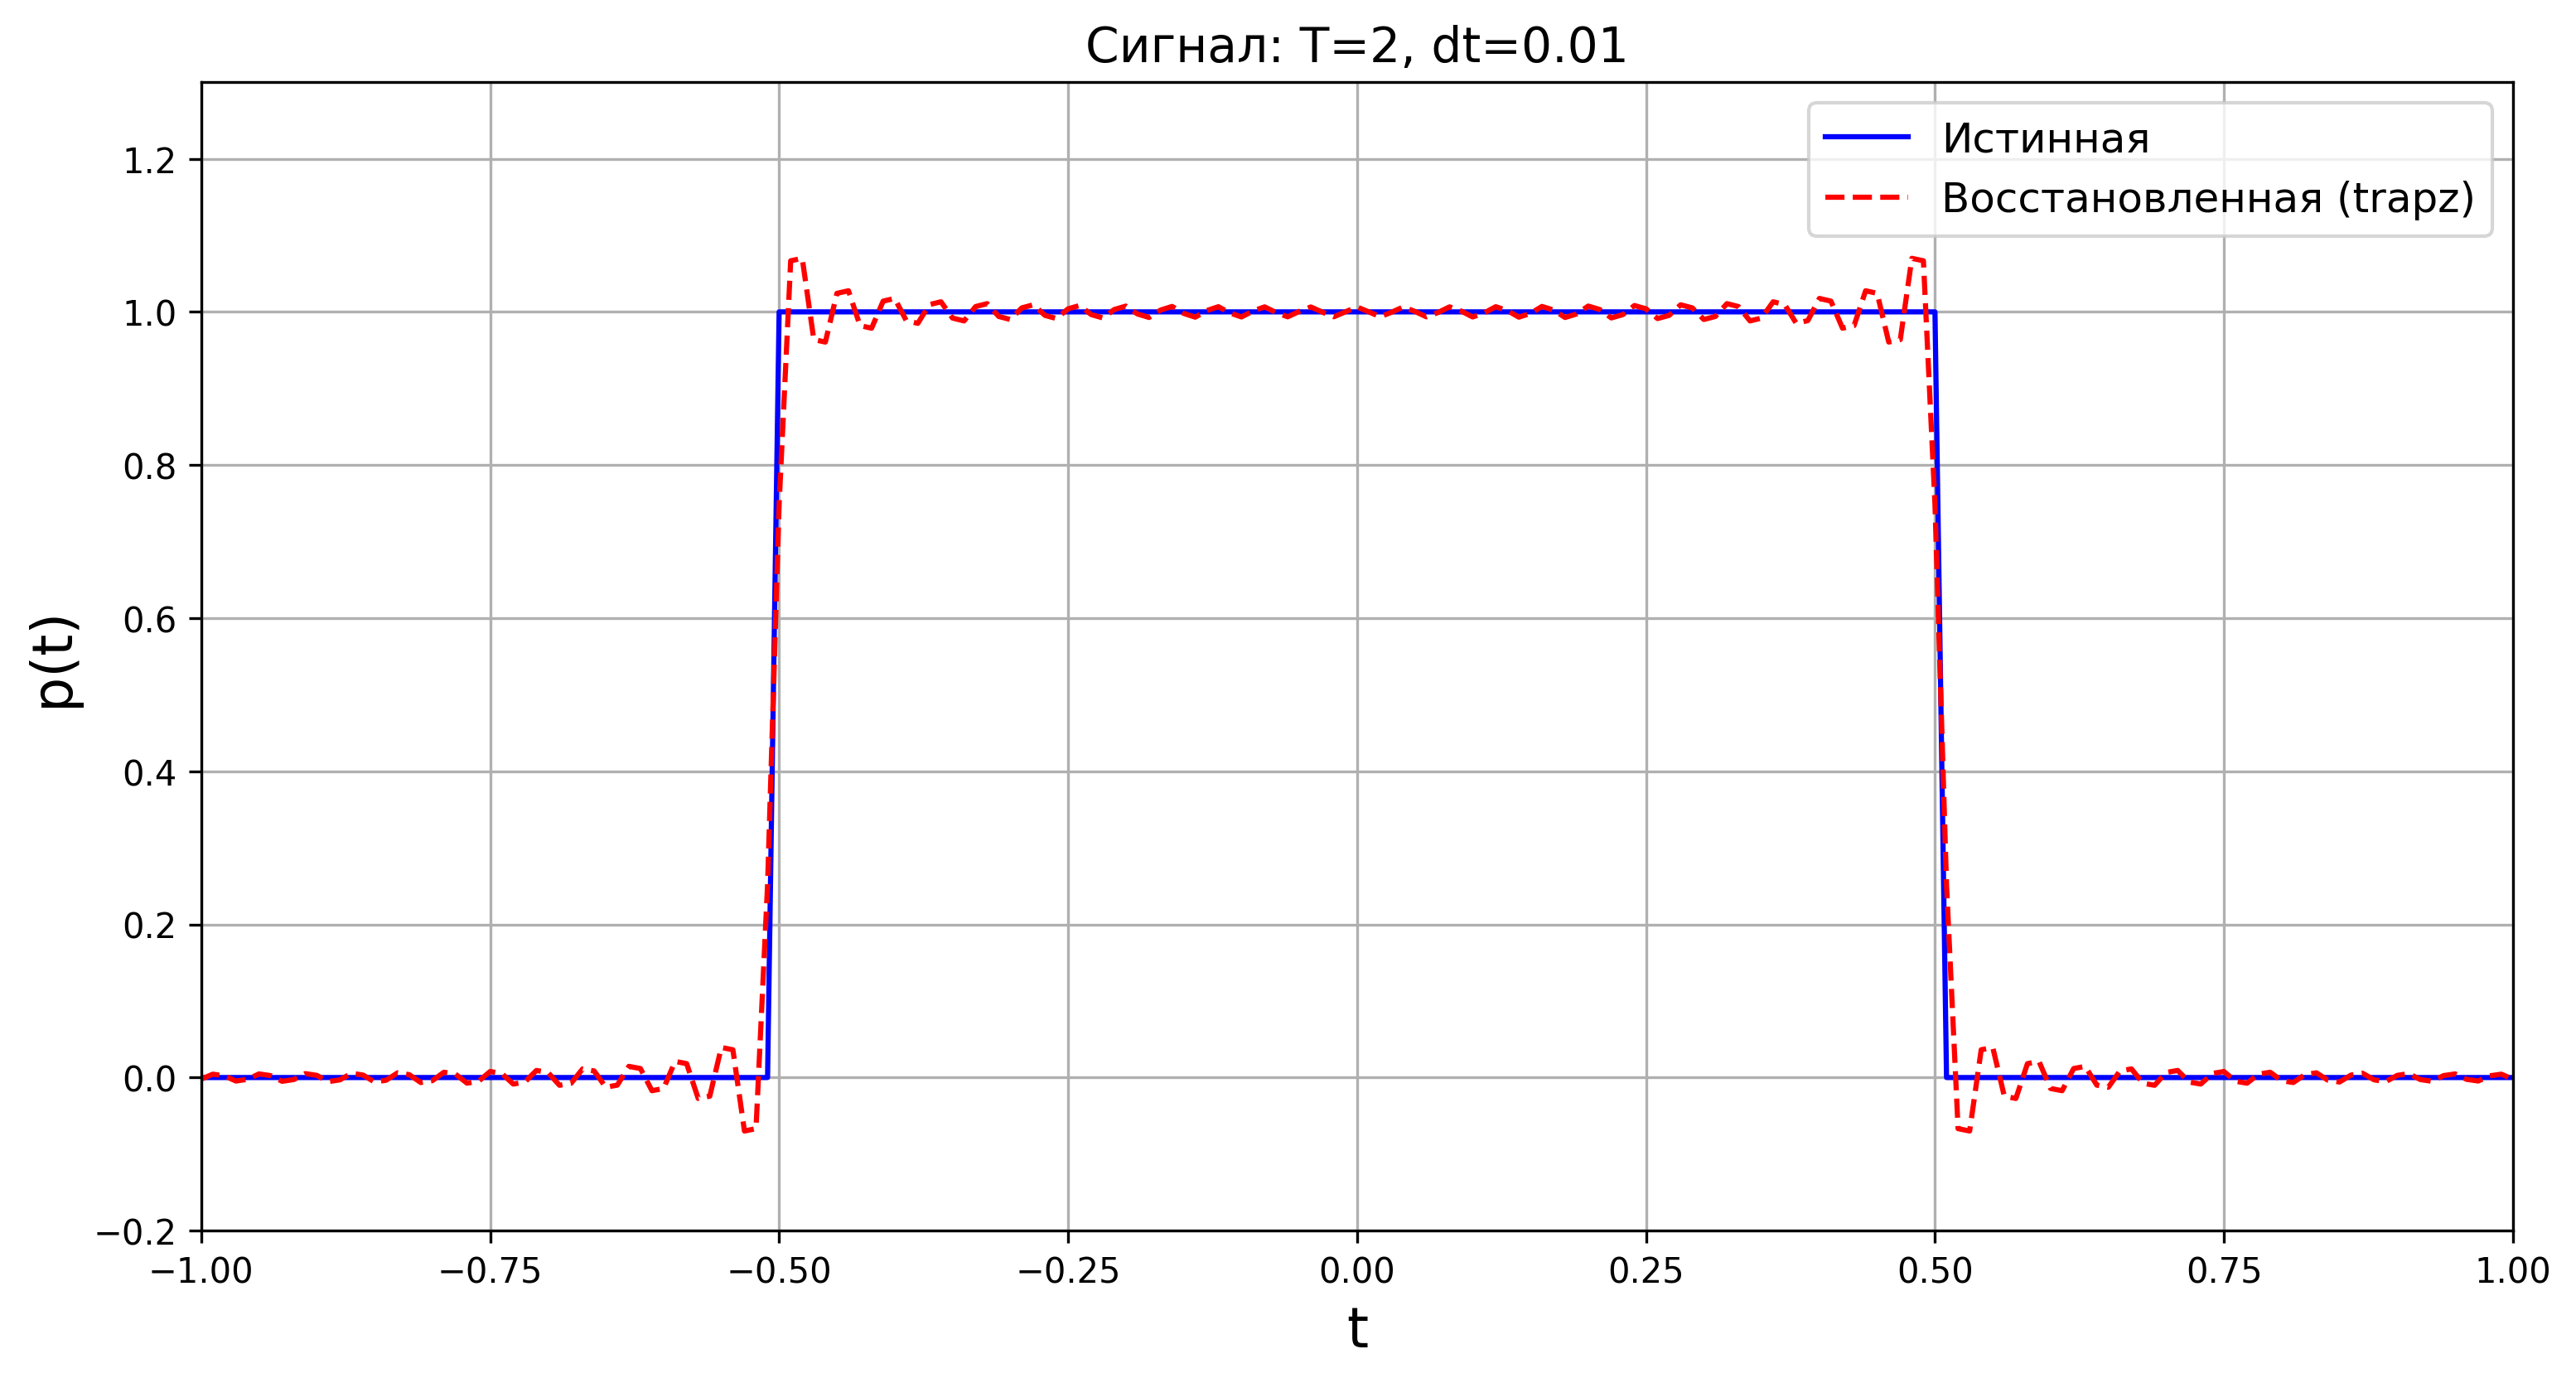
\includegraphics[width=0.95\textwidth]{Paper/images/T2_V50_dt0.010_dv0.001_signal.png}
    \caption{Сравнение исходной (синяя) и восстановленной (красная пунктир) функций.}
    \label{fig:signal_1}
\end{figure}

\begin{figure}[H]
    \centering
    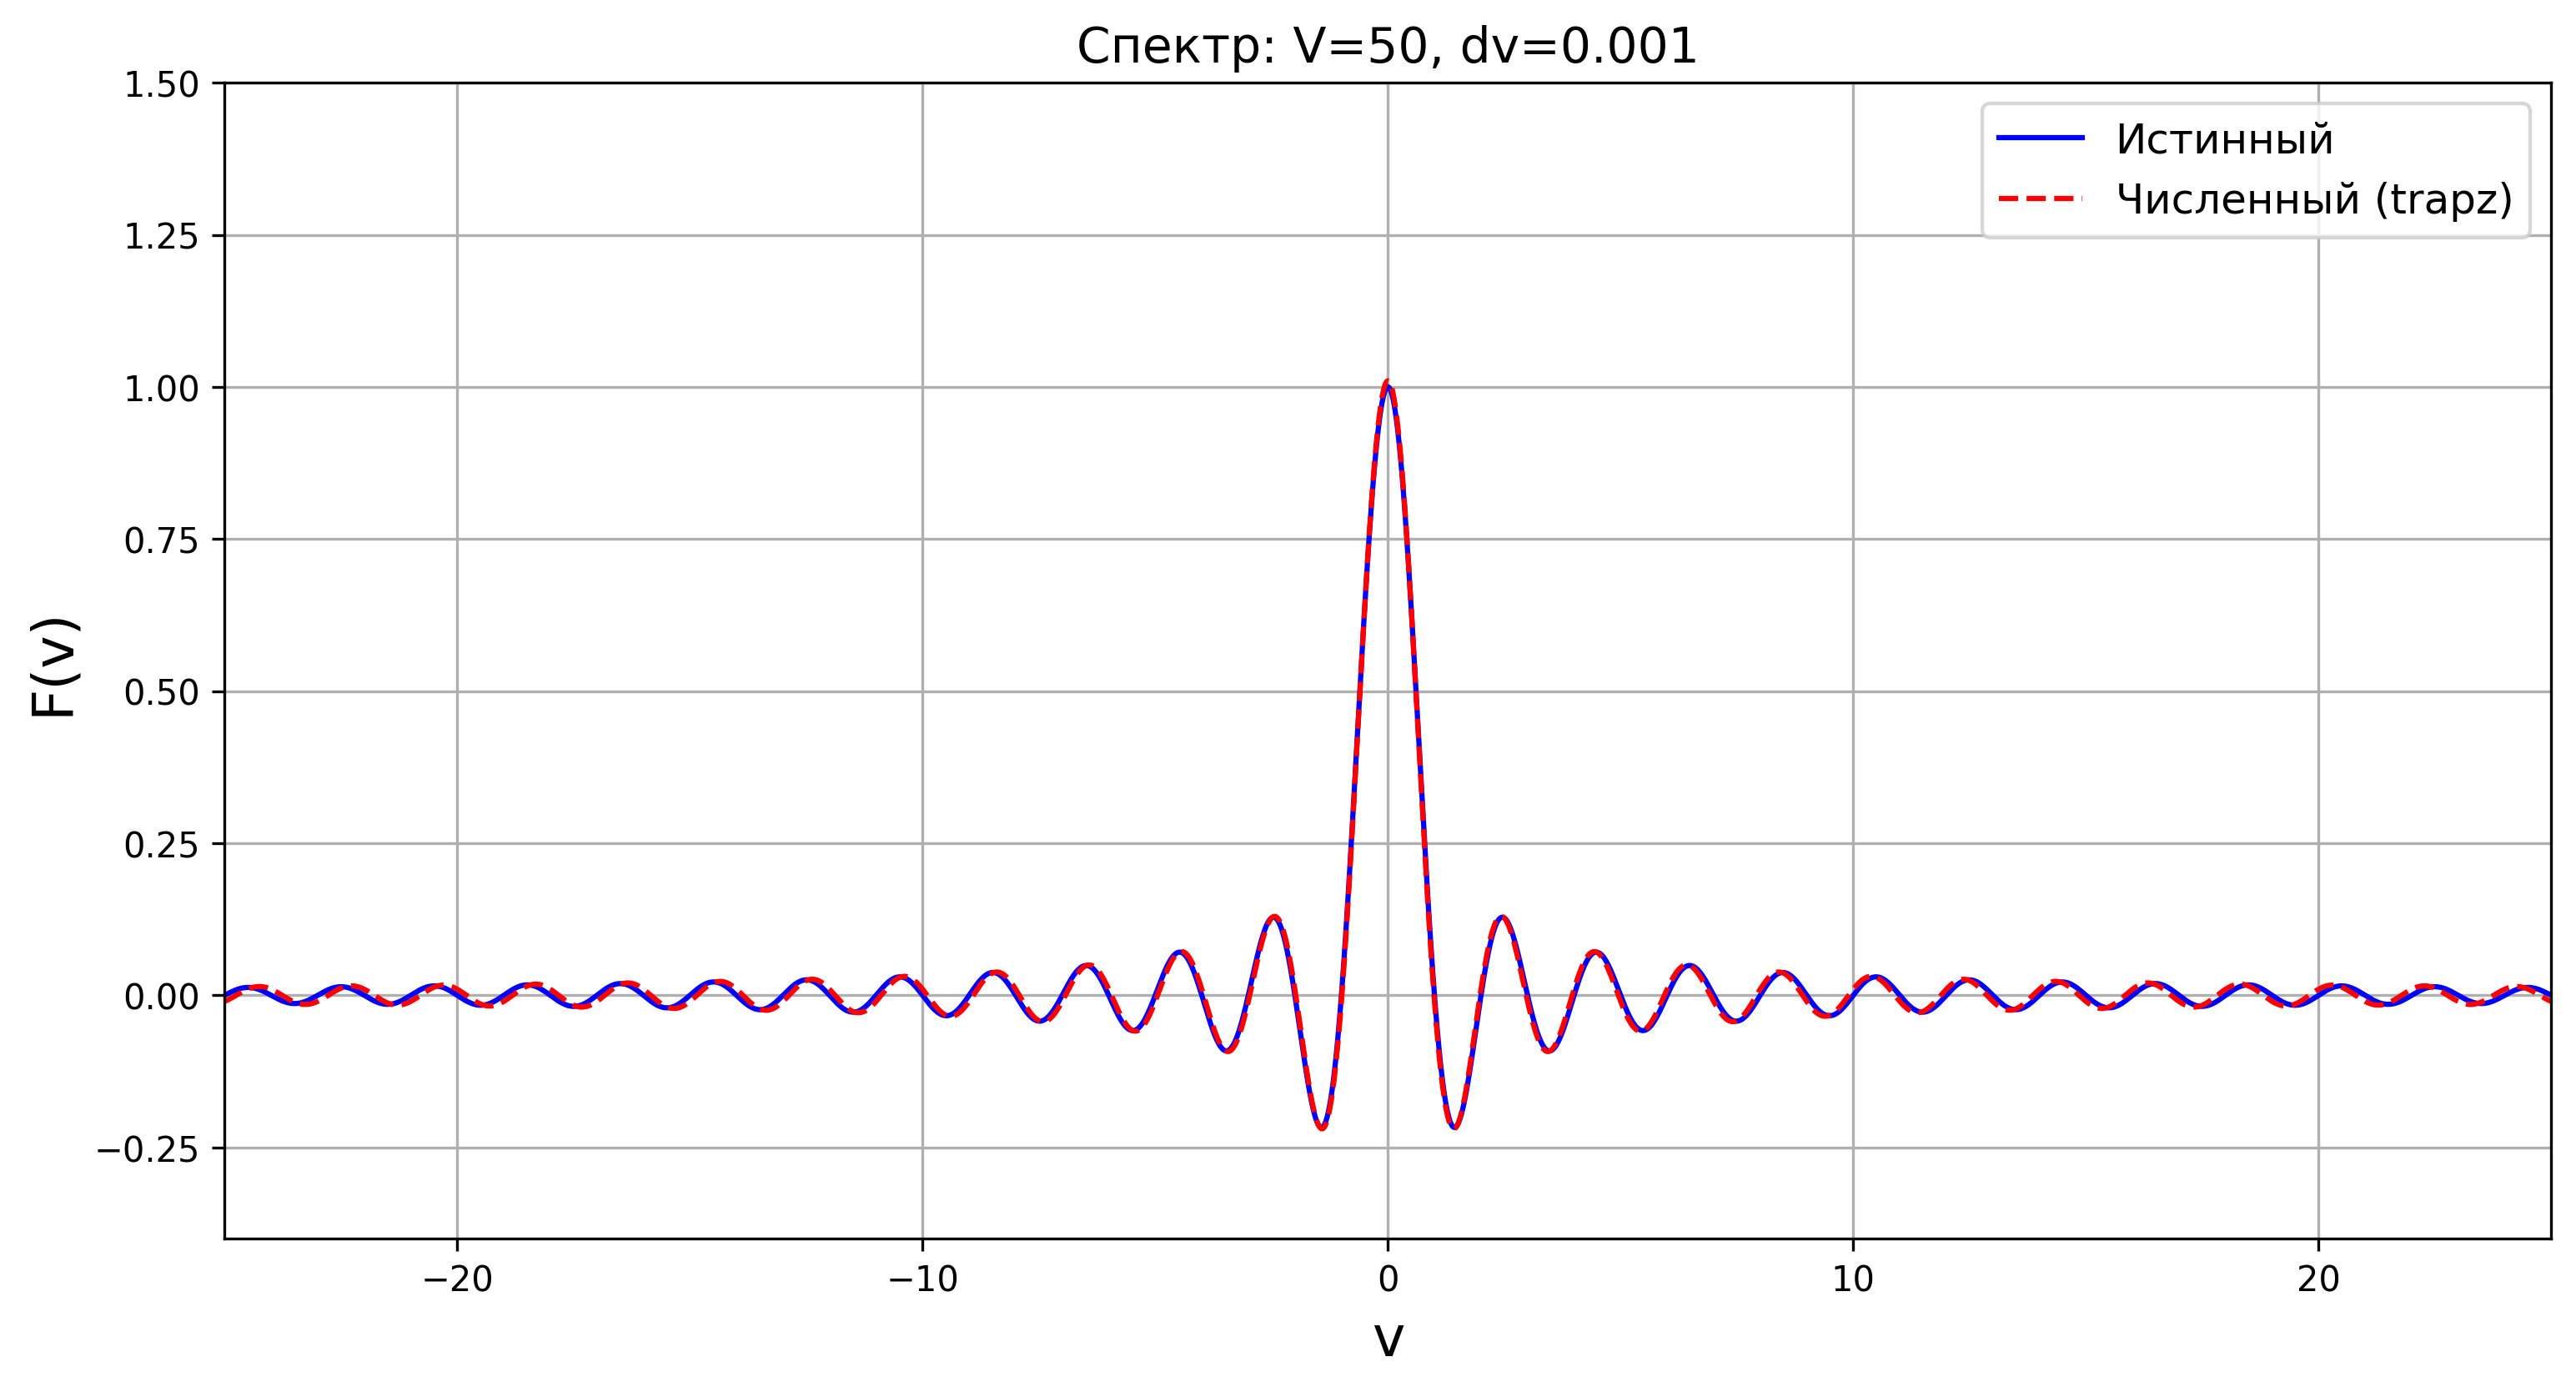
\includegraphics[width=0.95\textwidth]{Paper/images/T2_V50_dt0.010_dv0.001_spectrum.png}
    \caption{Сравнение истинного (синяя) и численного (красная пунктир) спектров.}
    \label{fig:spectrum_1}
\end{figure}


\newpage
\subsection{Комбинация 2: $T=4$, $V=100$, $dt=0.010$, $dv=0.001$}

\begin{figure}[H]
    \centering
    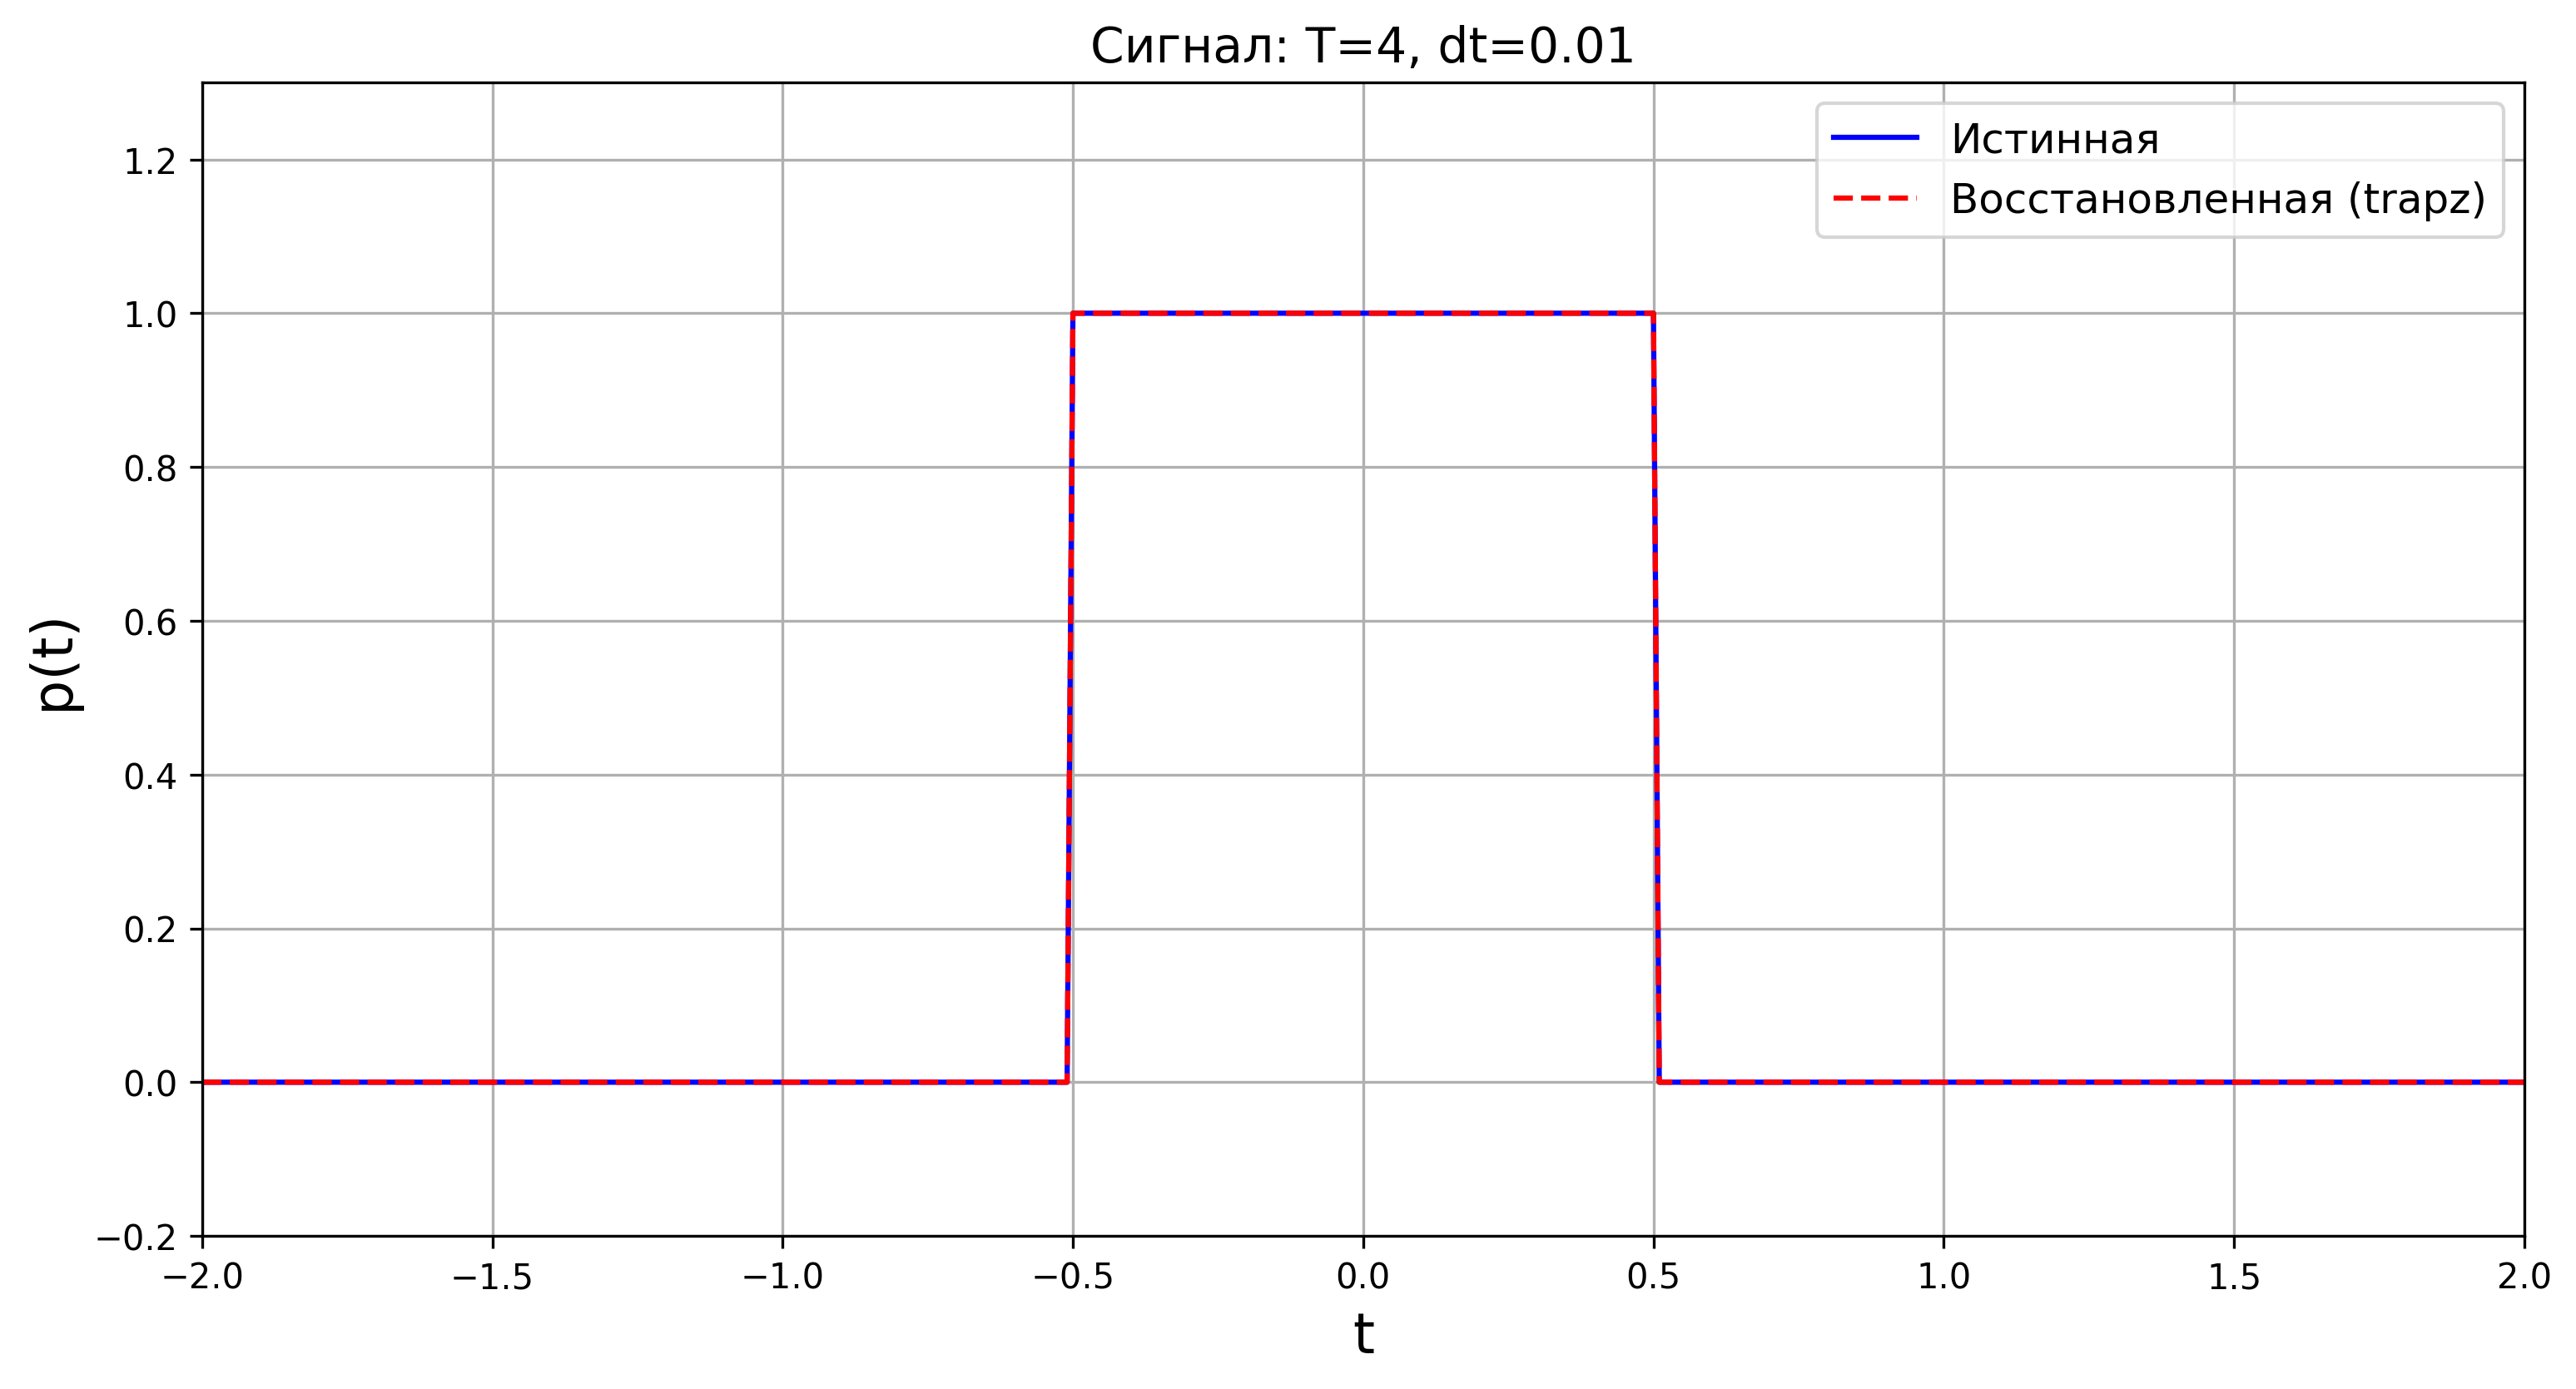
\includegraphics[width=0.95\textwidth]{Paper/images/T4_V100_dt0.010_dv0.001_signal.png}
    \caption{Сравнение исходной (синяя) и восстановленной (красная пунктир) функций.}
    \label{fig:signal_2}
\end{figure}

\begin{figure}[H]
    \centering
    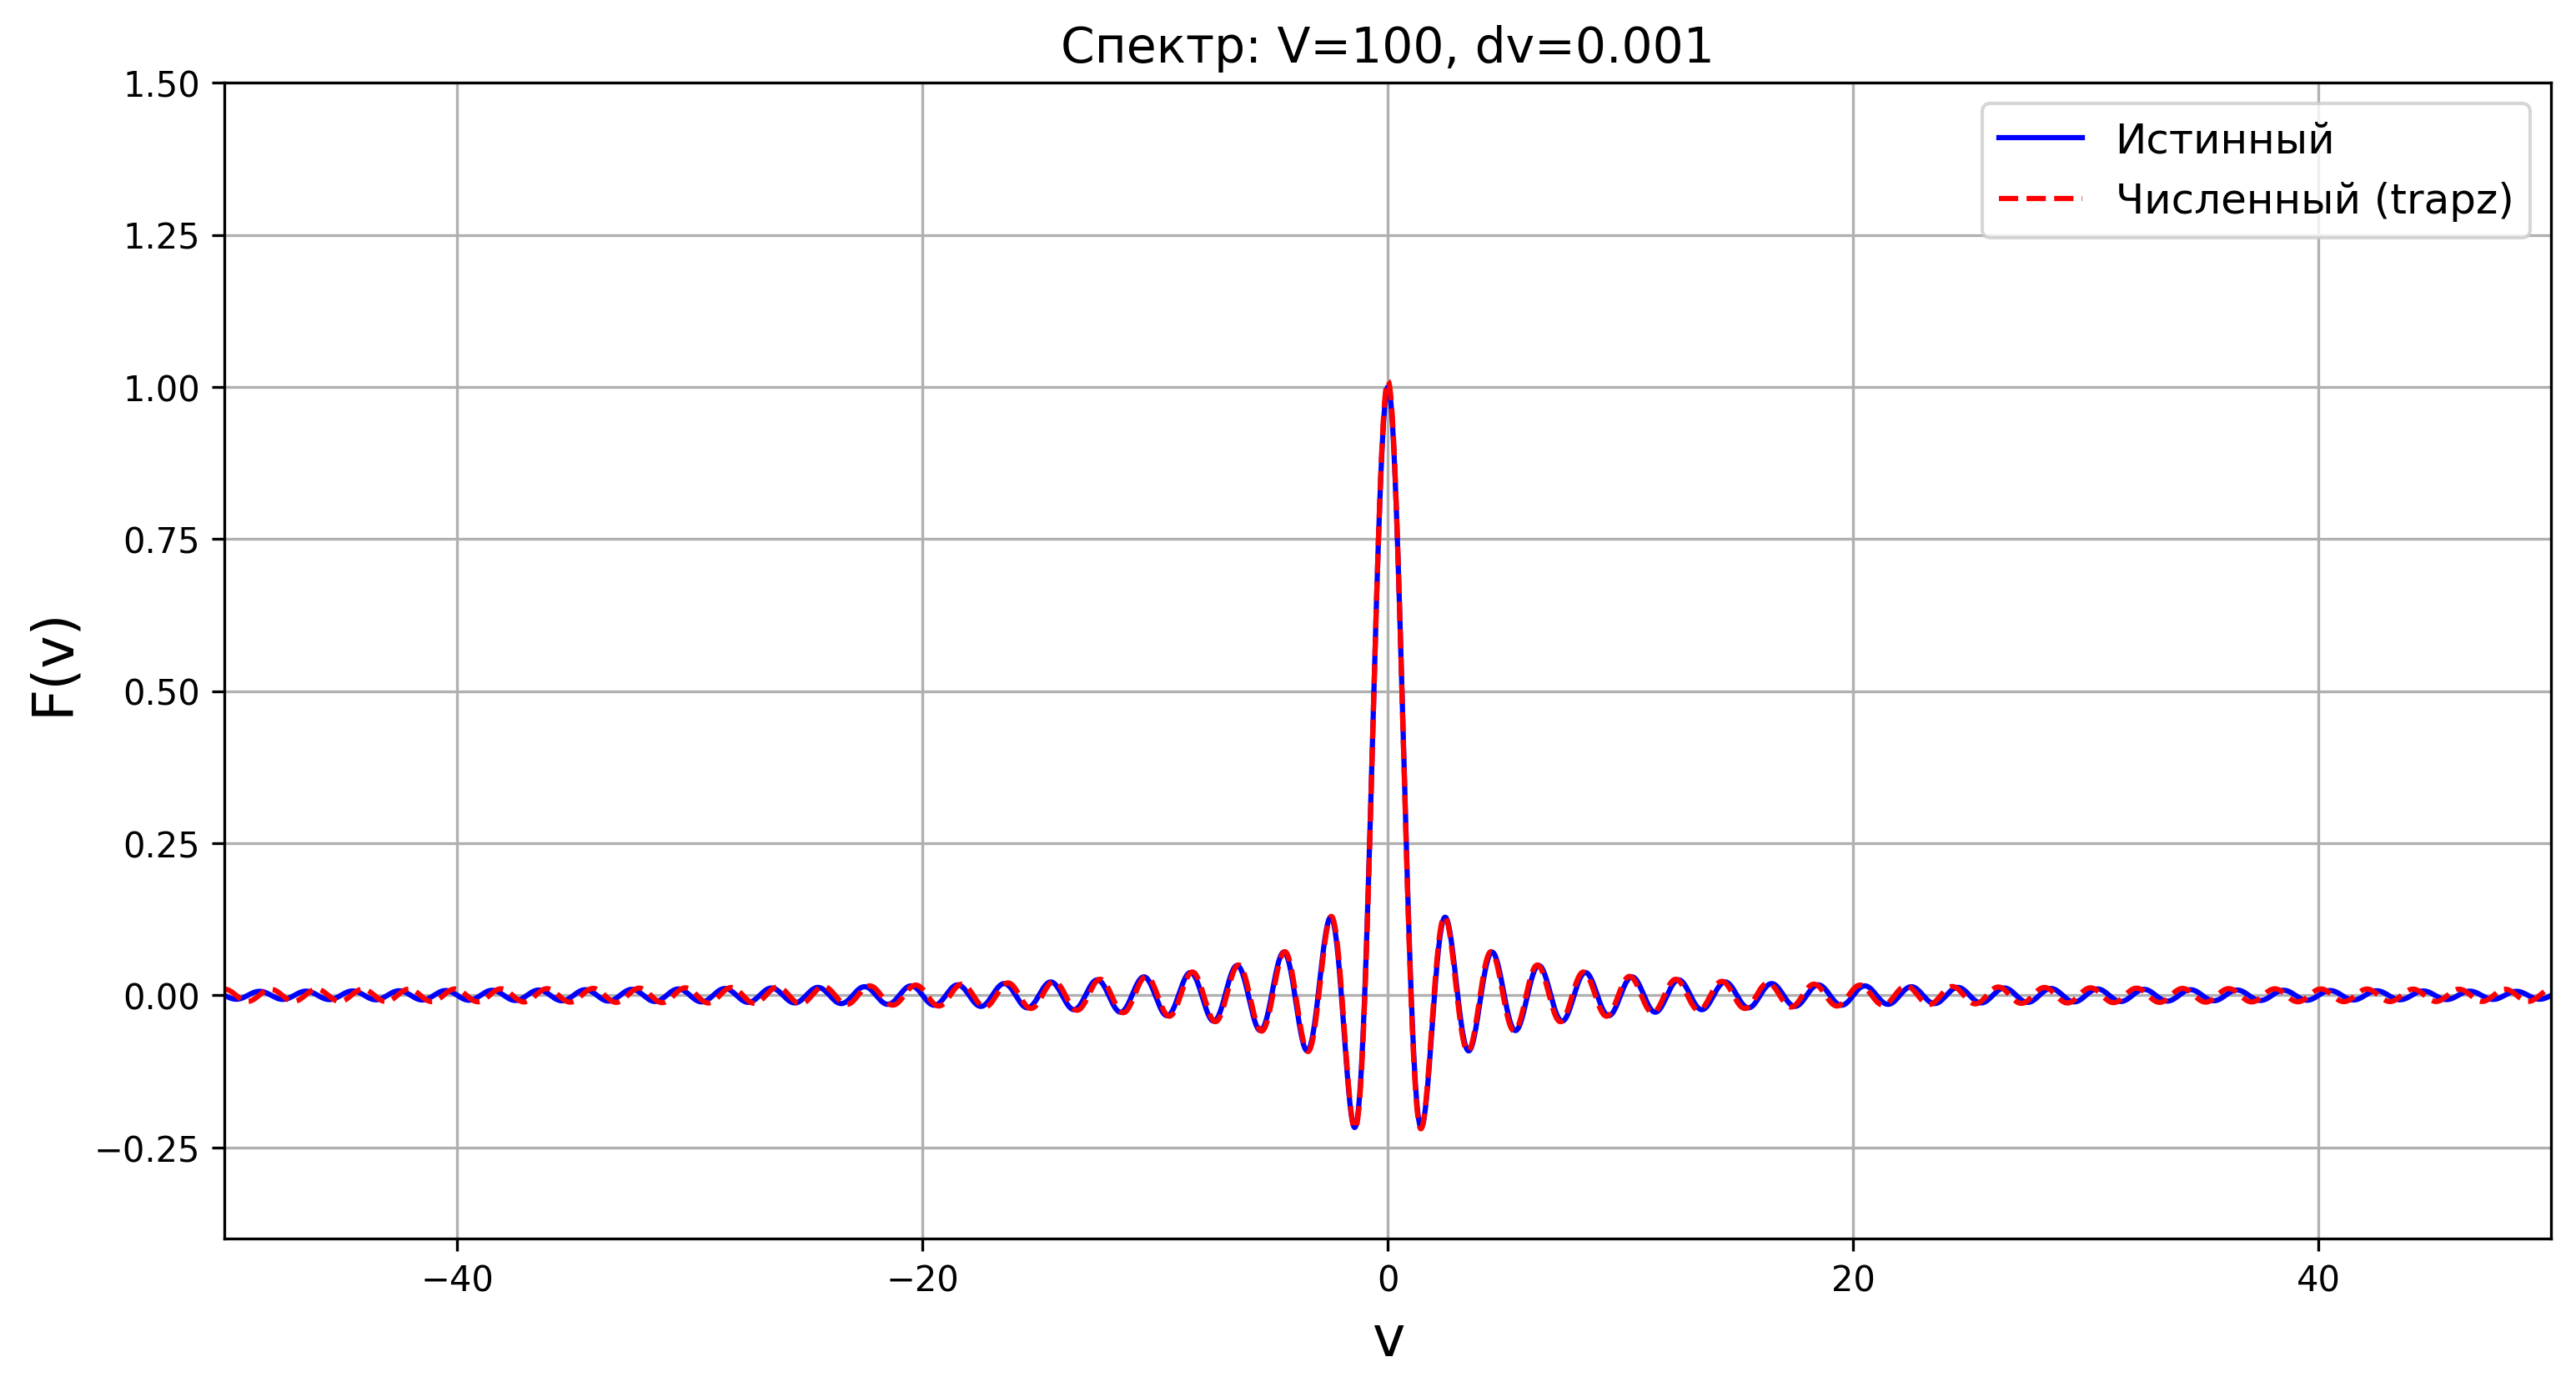
\includegraphics[width=0.95\textwidth]{Paper/images/T4_V100_dt0.010_dv0.001_spectrum.png}
    \caption{Сравнение истинного (синяя) и численного (красная пунктир) спектров.}
    \label{fig:spectrum_2}
\end{figure}


\newpage
\subsection{Комбинация 3: $T=8$, $V=200$, $dt=0.010$, $dv=0.001$}

\begin{figure}[H]
    \centering
    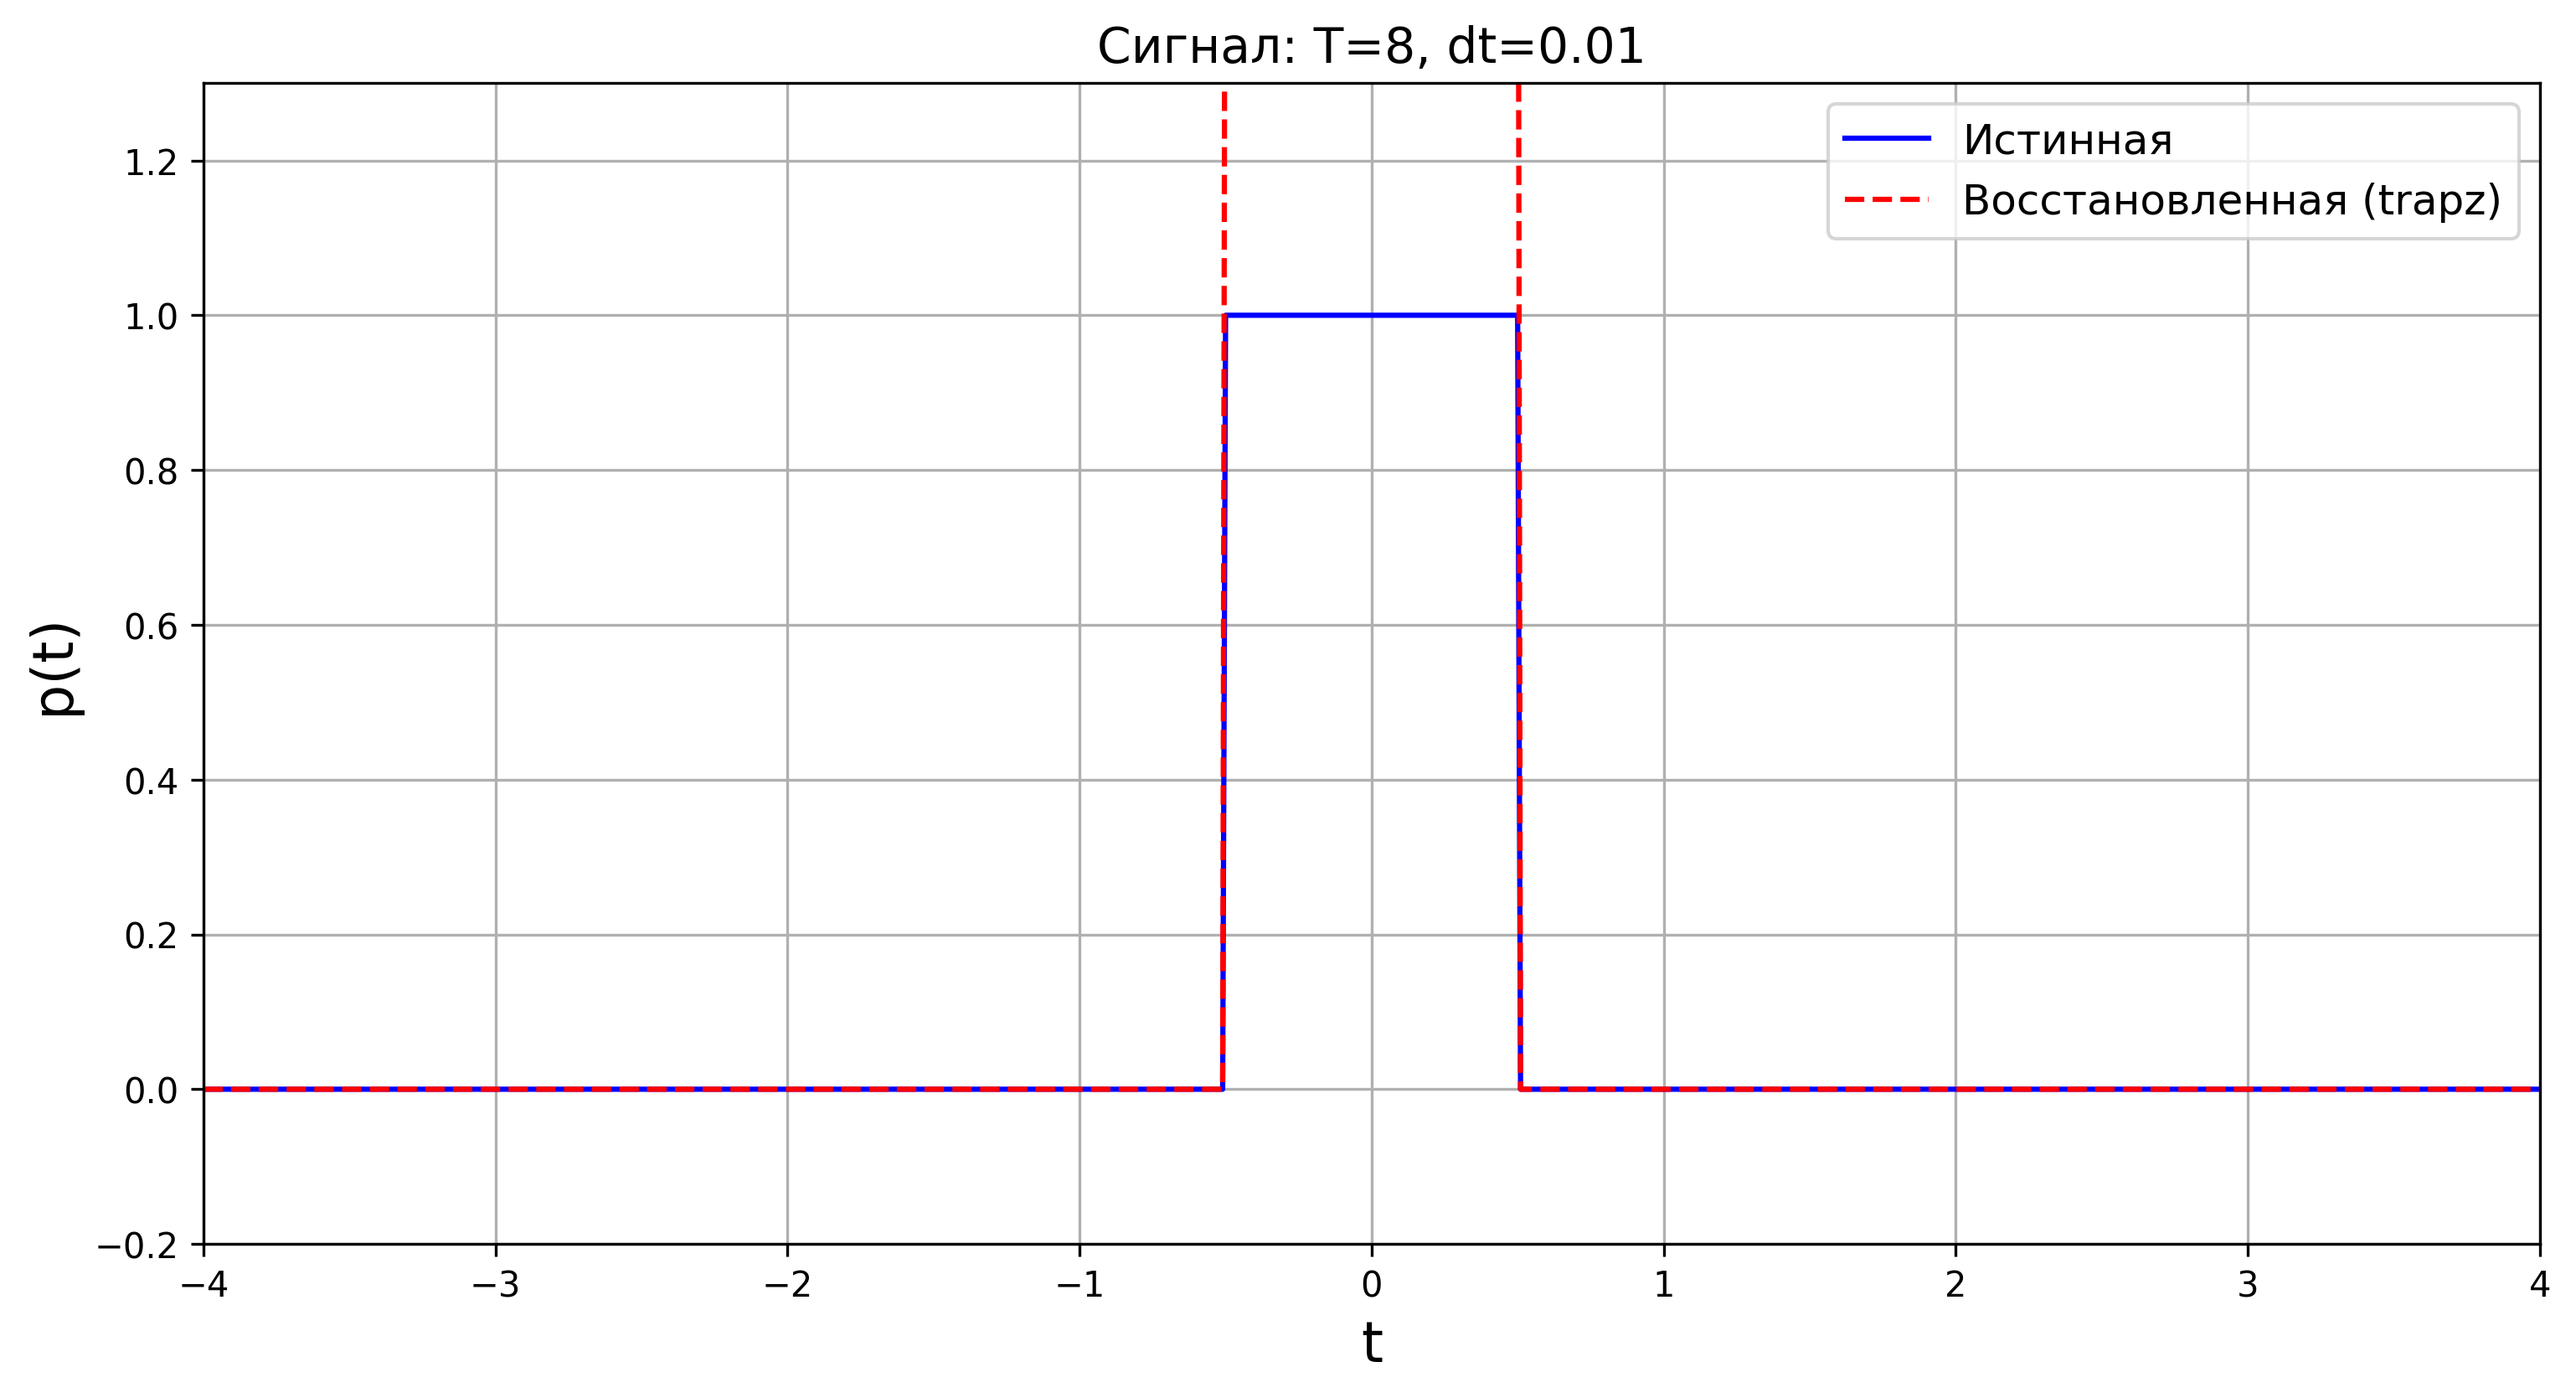
\includegraphics[width=0.95\textwidth]{Paper/images/T8_V200_dt0.010_dv0.001_signal.png}
    \caption{Сравнение исходной (синяя) и восстановленной (красная пунктир) функций.}
    \label{fig:signal_3}
\end{figure}

\begin{figure}[H]
    \centering
    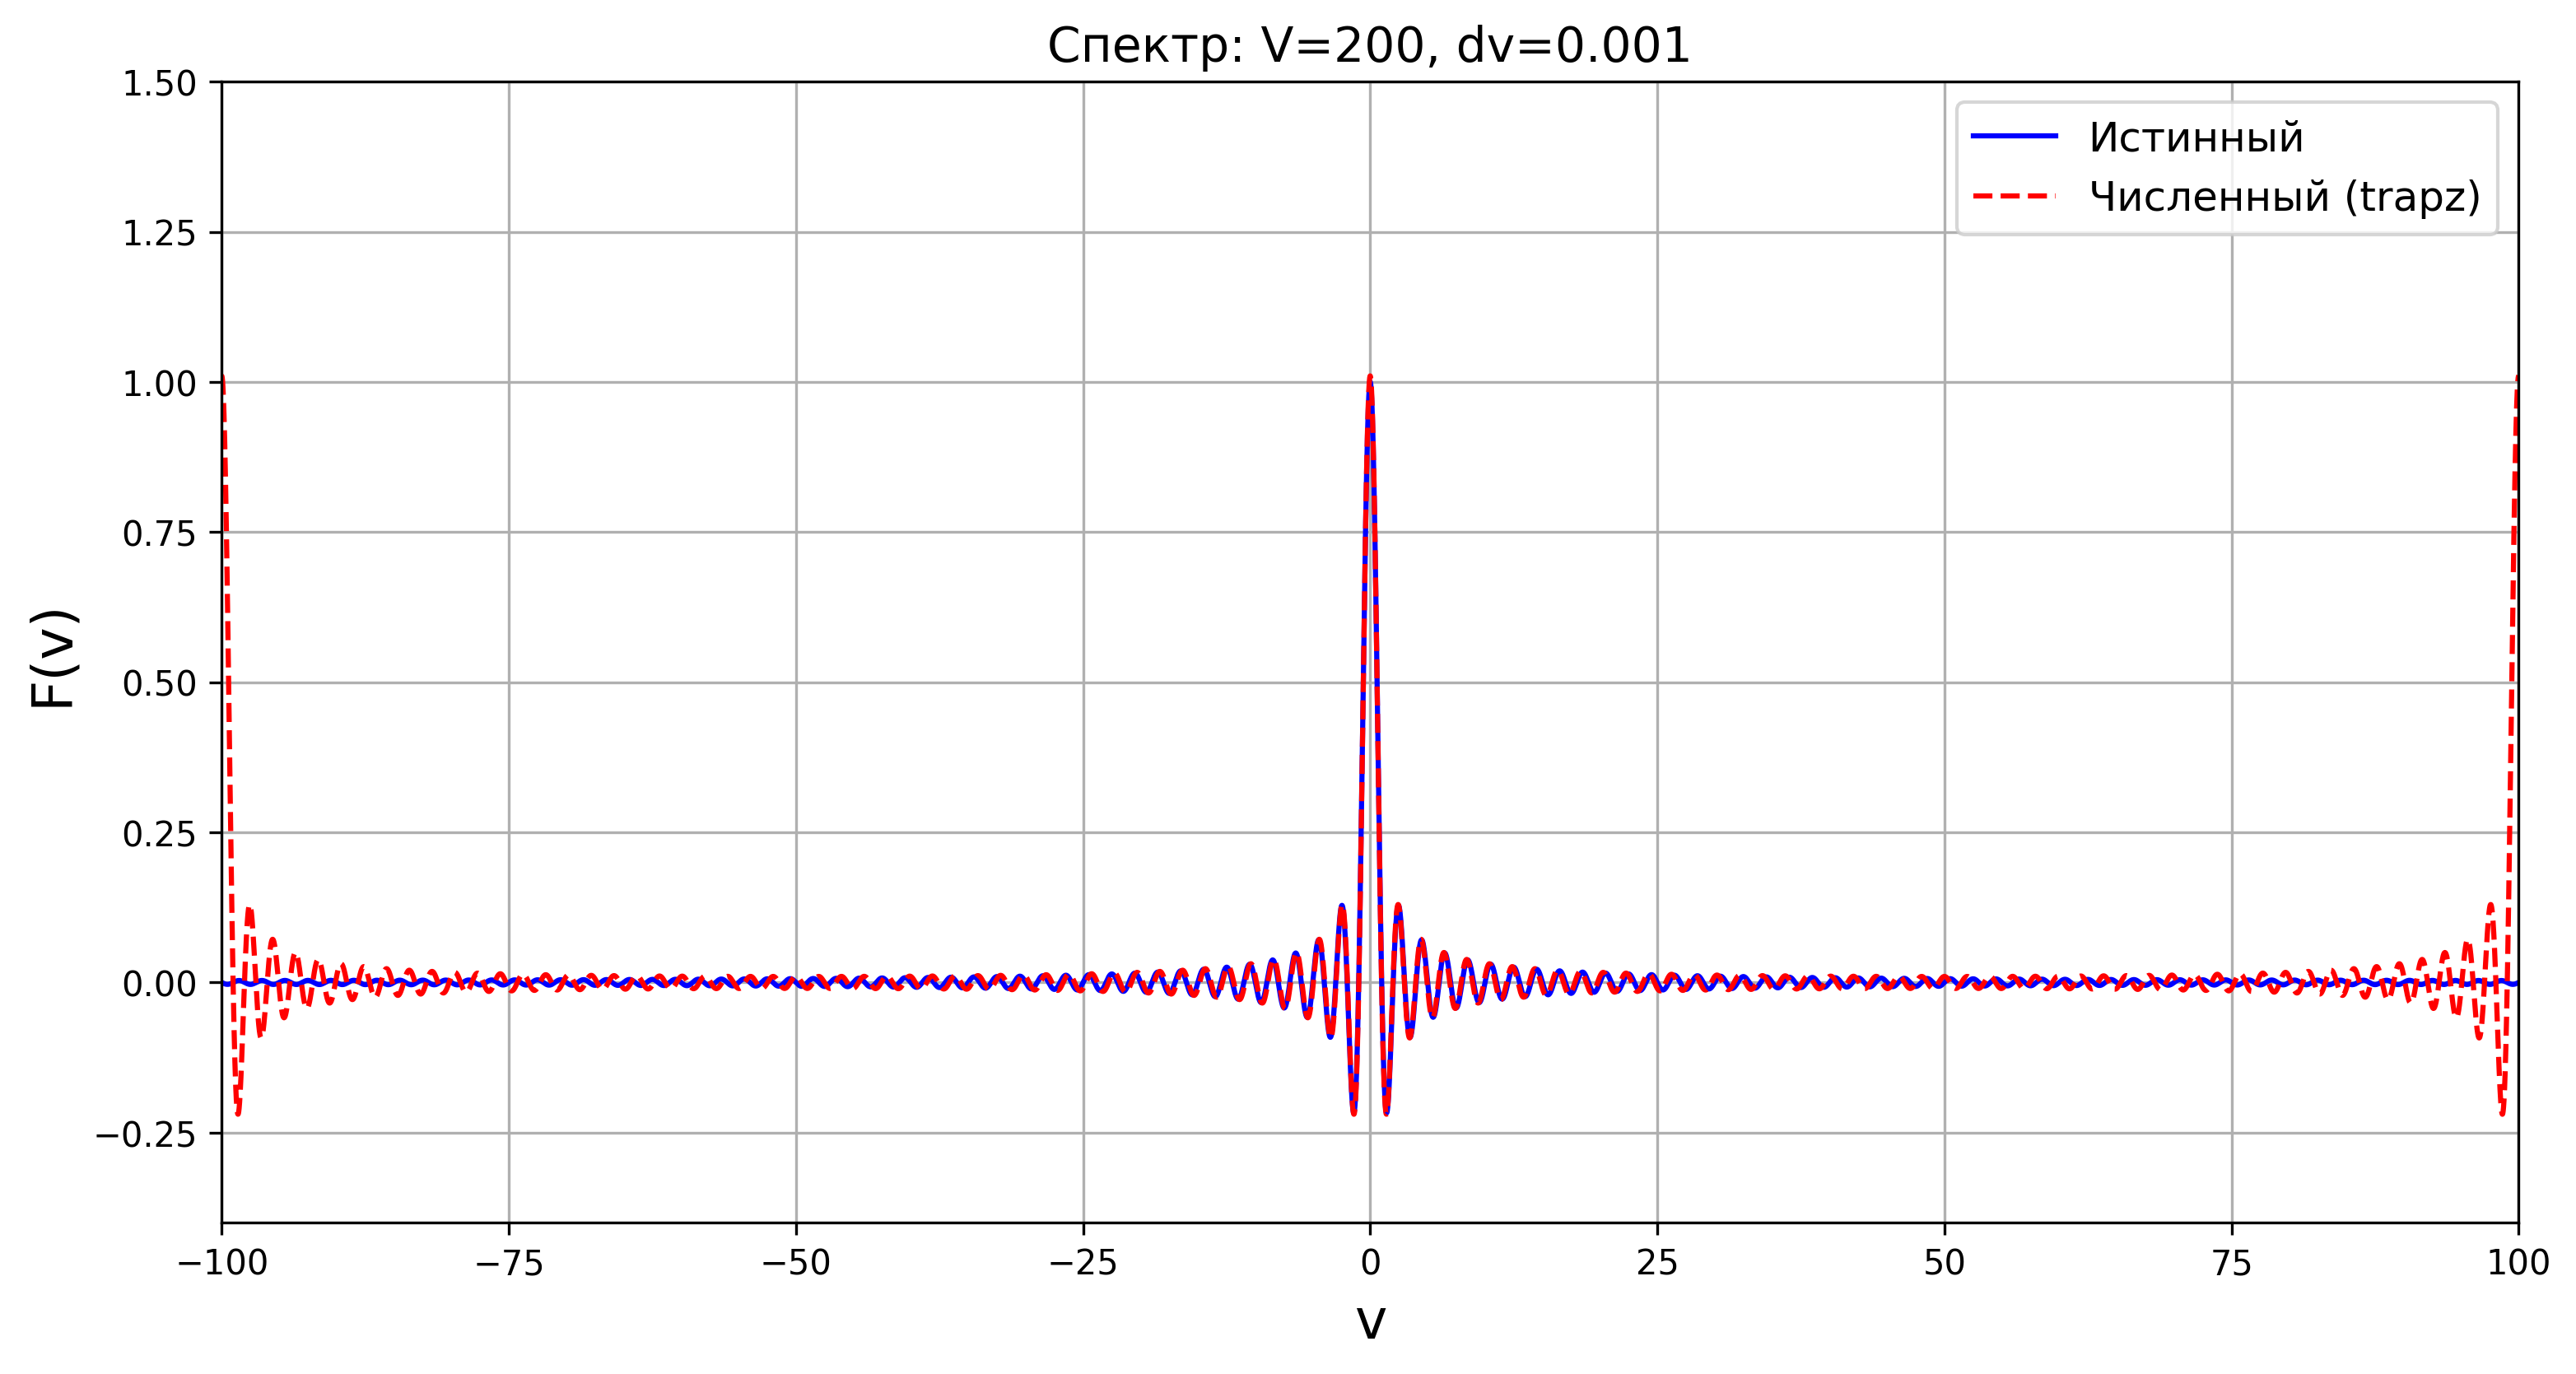
\includegraphics[width=0.95\textwidth]{Paper/images/T8_V200_dt0.010_dv0.001_spectrum.png}
    \caption{Сравнение истинного (синяя) и численного (красная пунктир) спектров.}
    \label{fig:spectrum_3}
\end{figure}


\newpage
\subsection{Комбинация 4: $T=2$, $V=50$, $dt=0.050$, $dv=0.500$}

\begin{figure}[H]
    \centering
    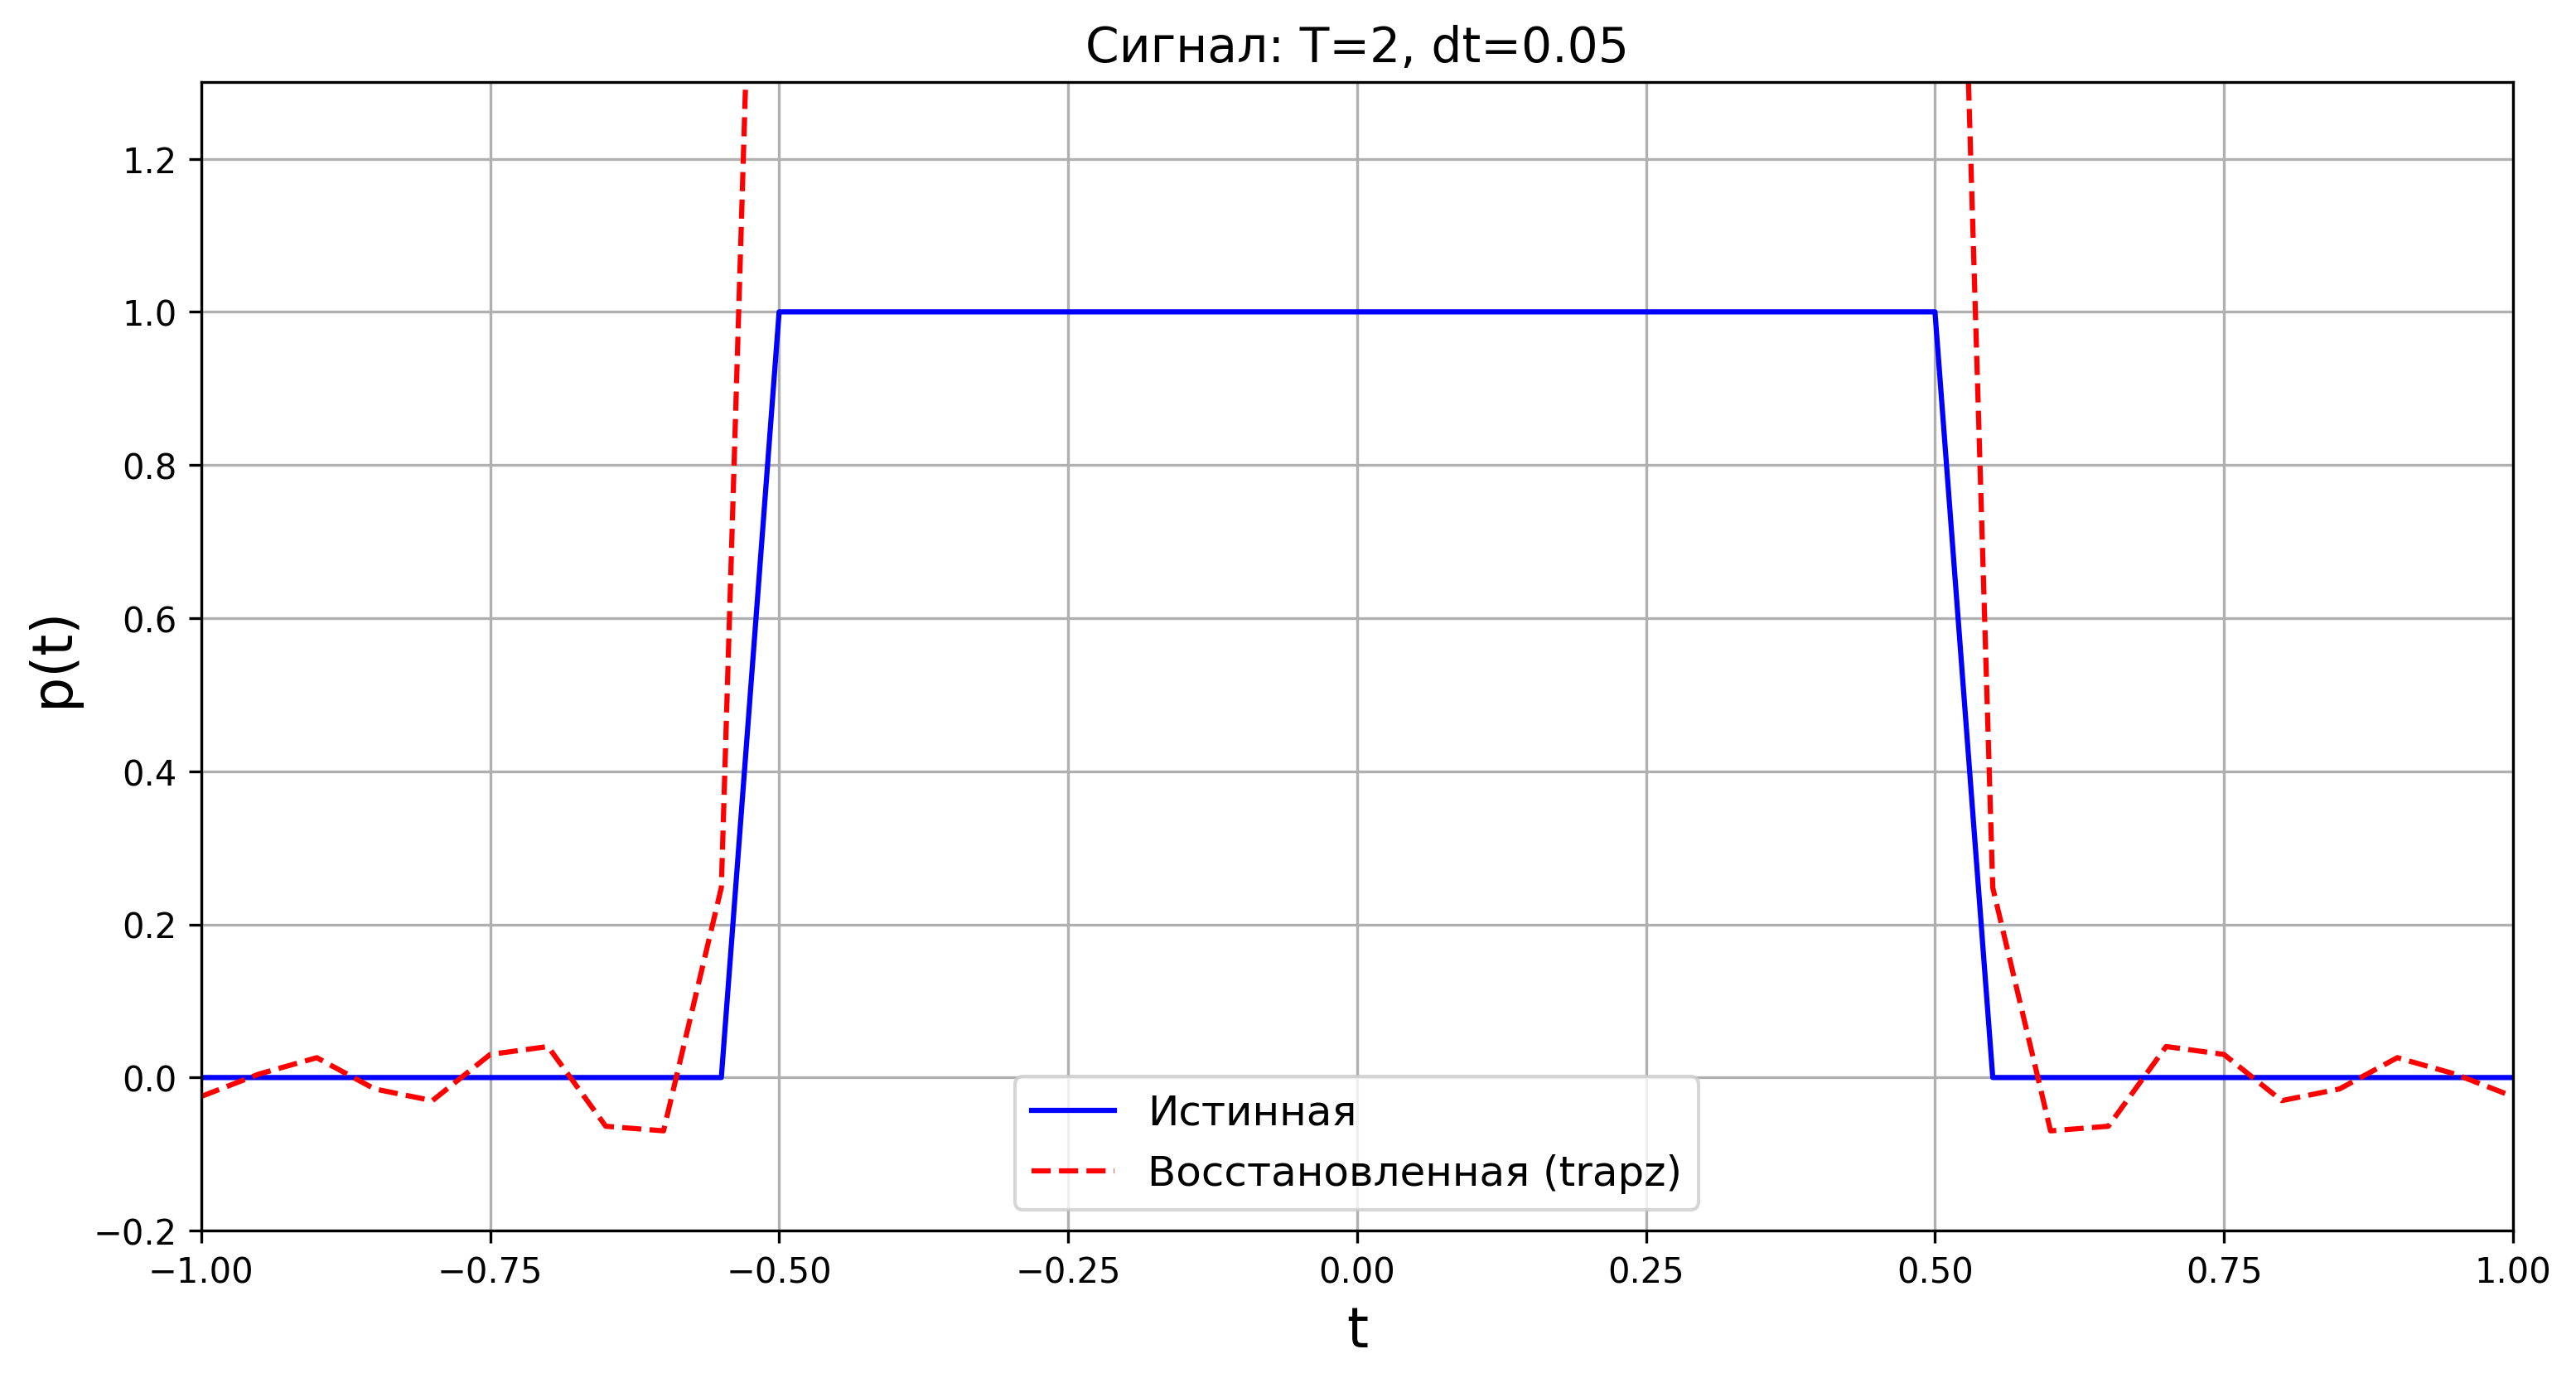
\includegraphics[width=0.95\textwidth]{Paper/images/T2_V50_dt0.050_dv0.500_signal.png}
    \caption{Сравнение исходной (синяя) и восстановленной (красная пунктир) функций.}
    \label{fig:signal_4}
\end{figure}

\begin{figure}[H]
    \centering
    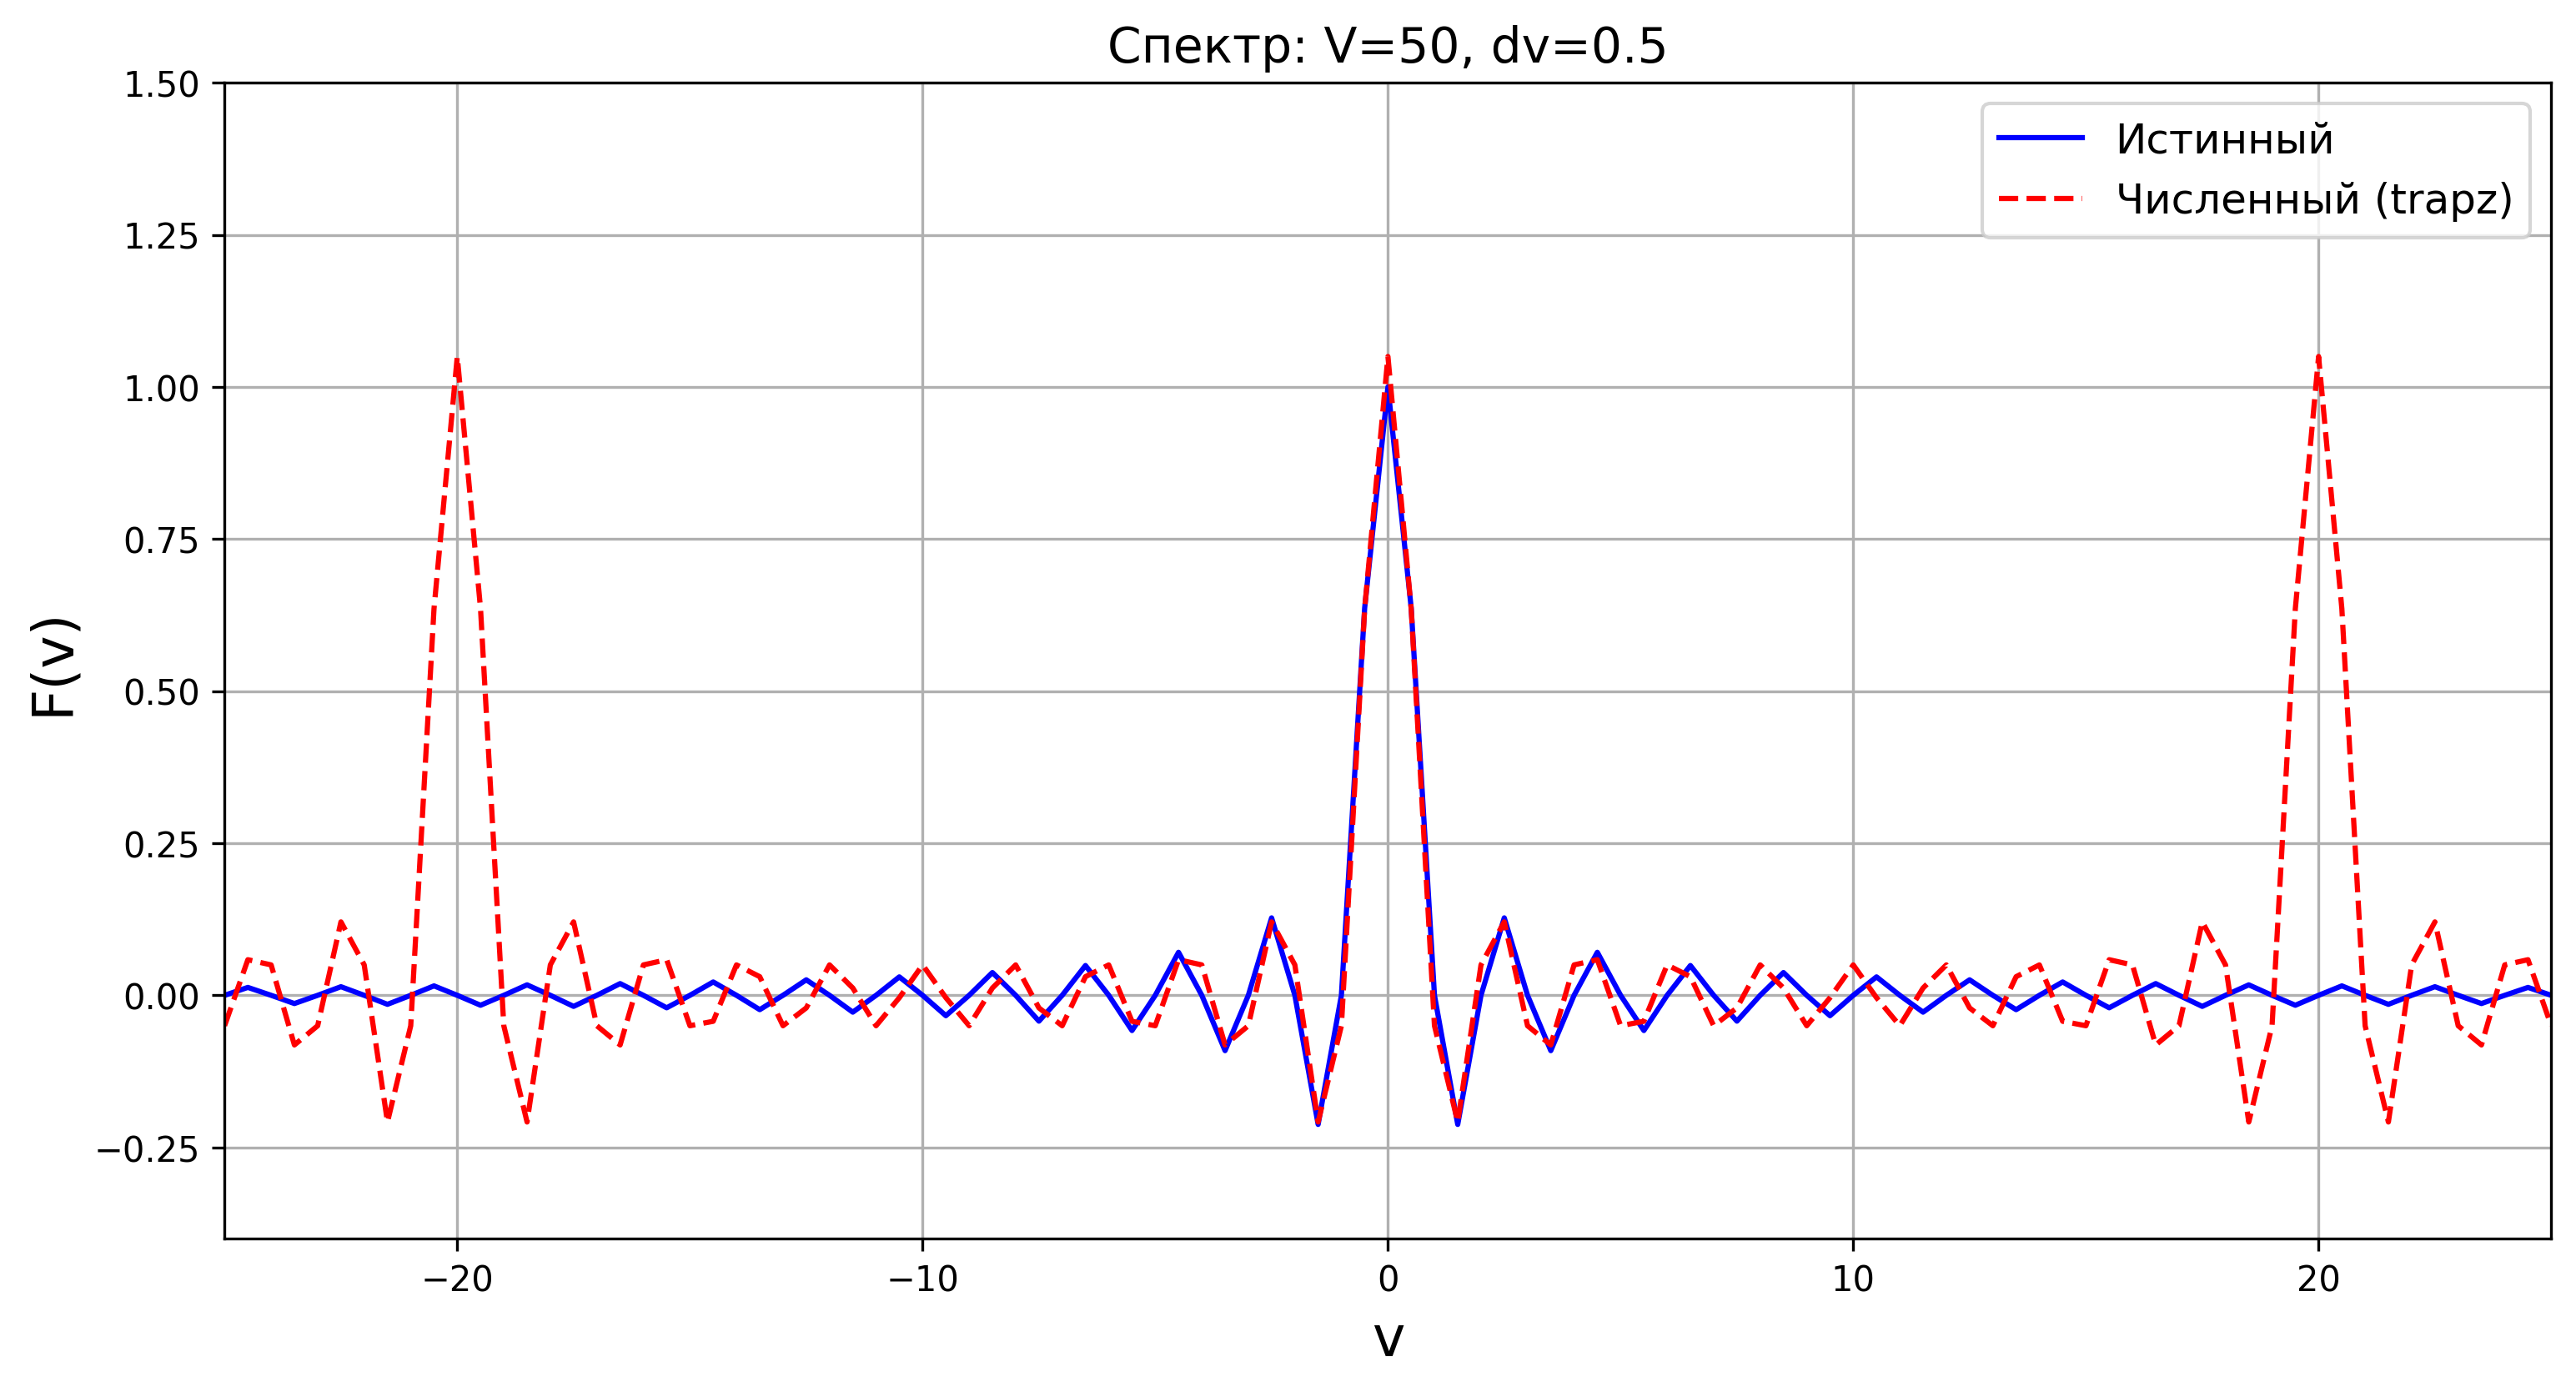
\includegraphics[width=0.95\textwidth]{Paper/images/T2_V50_dt0.050_dv0.500_spectrum.png}
    \caption{Сравнение истинного (синяя) и численного (красная пунктир) спектров.}
    \label{fig:spectrum_4}
\end{figure}


\newpage
\subsection{Комбинация 5: $T=4$, $V=100$, $dt=0.050$, $dv=0.500$}

\begin{figure}[H]
    \centering
    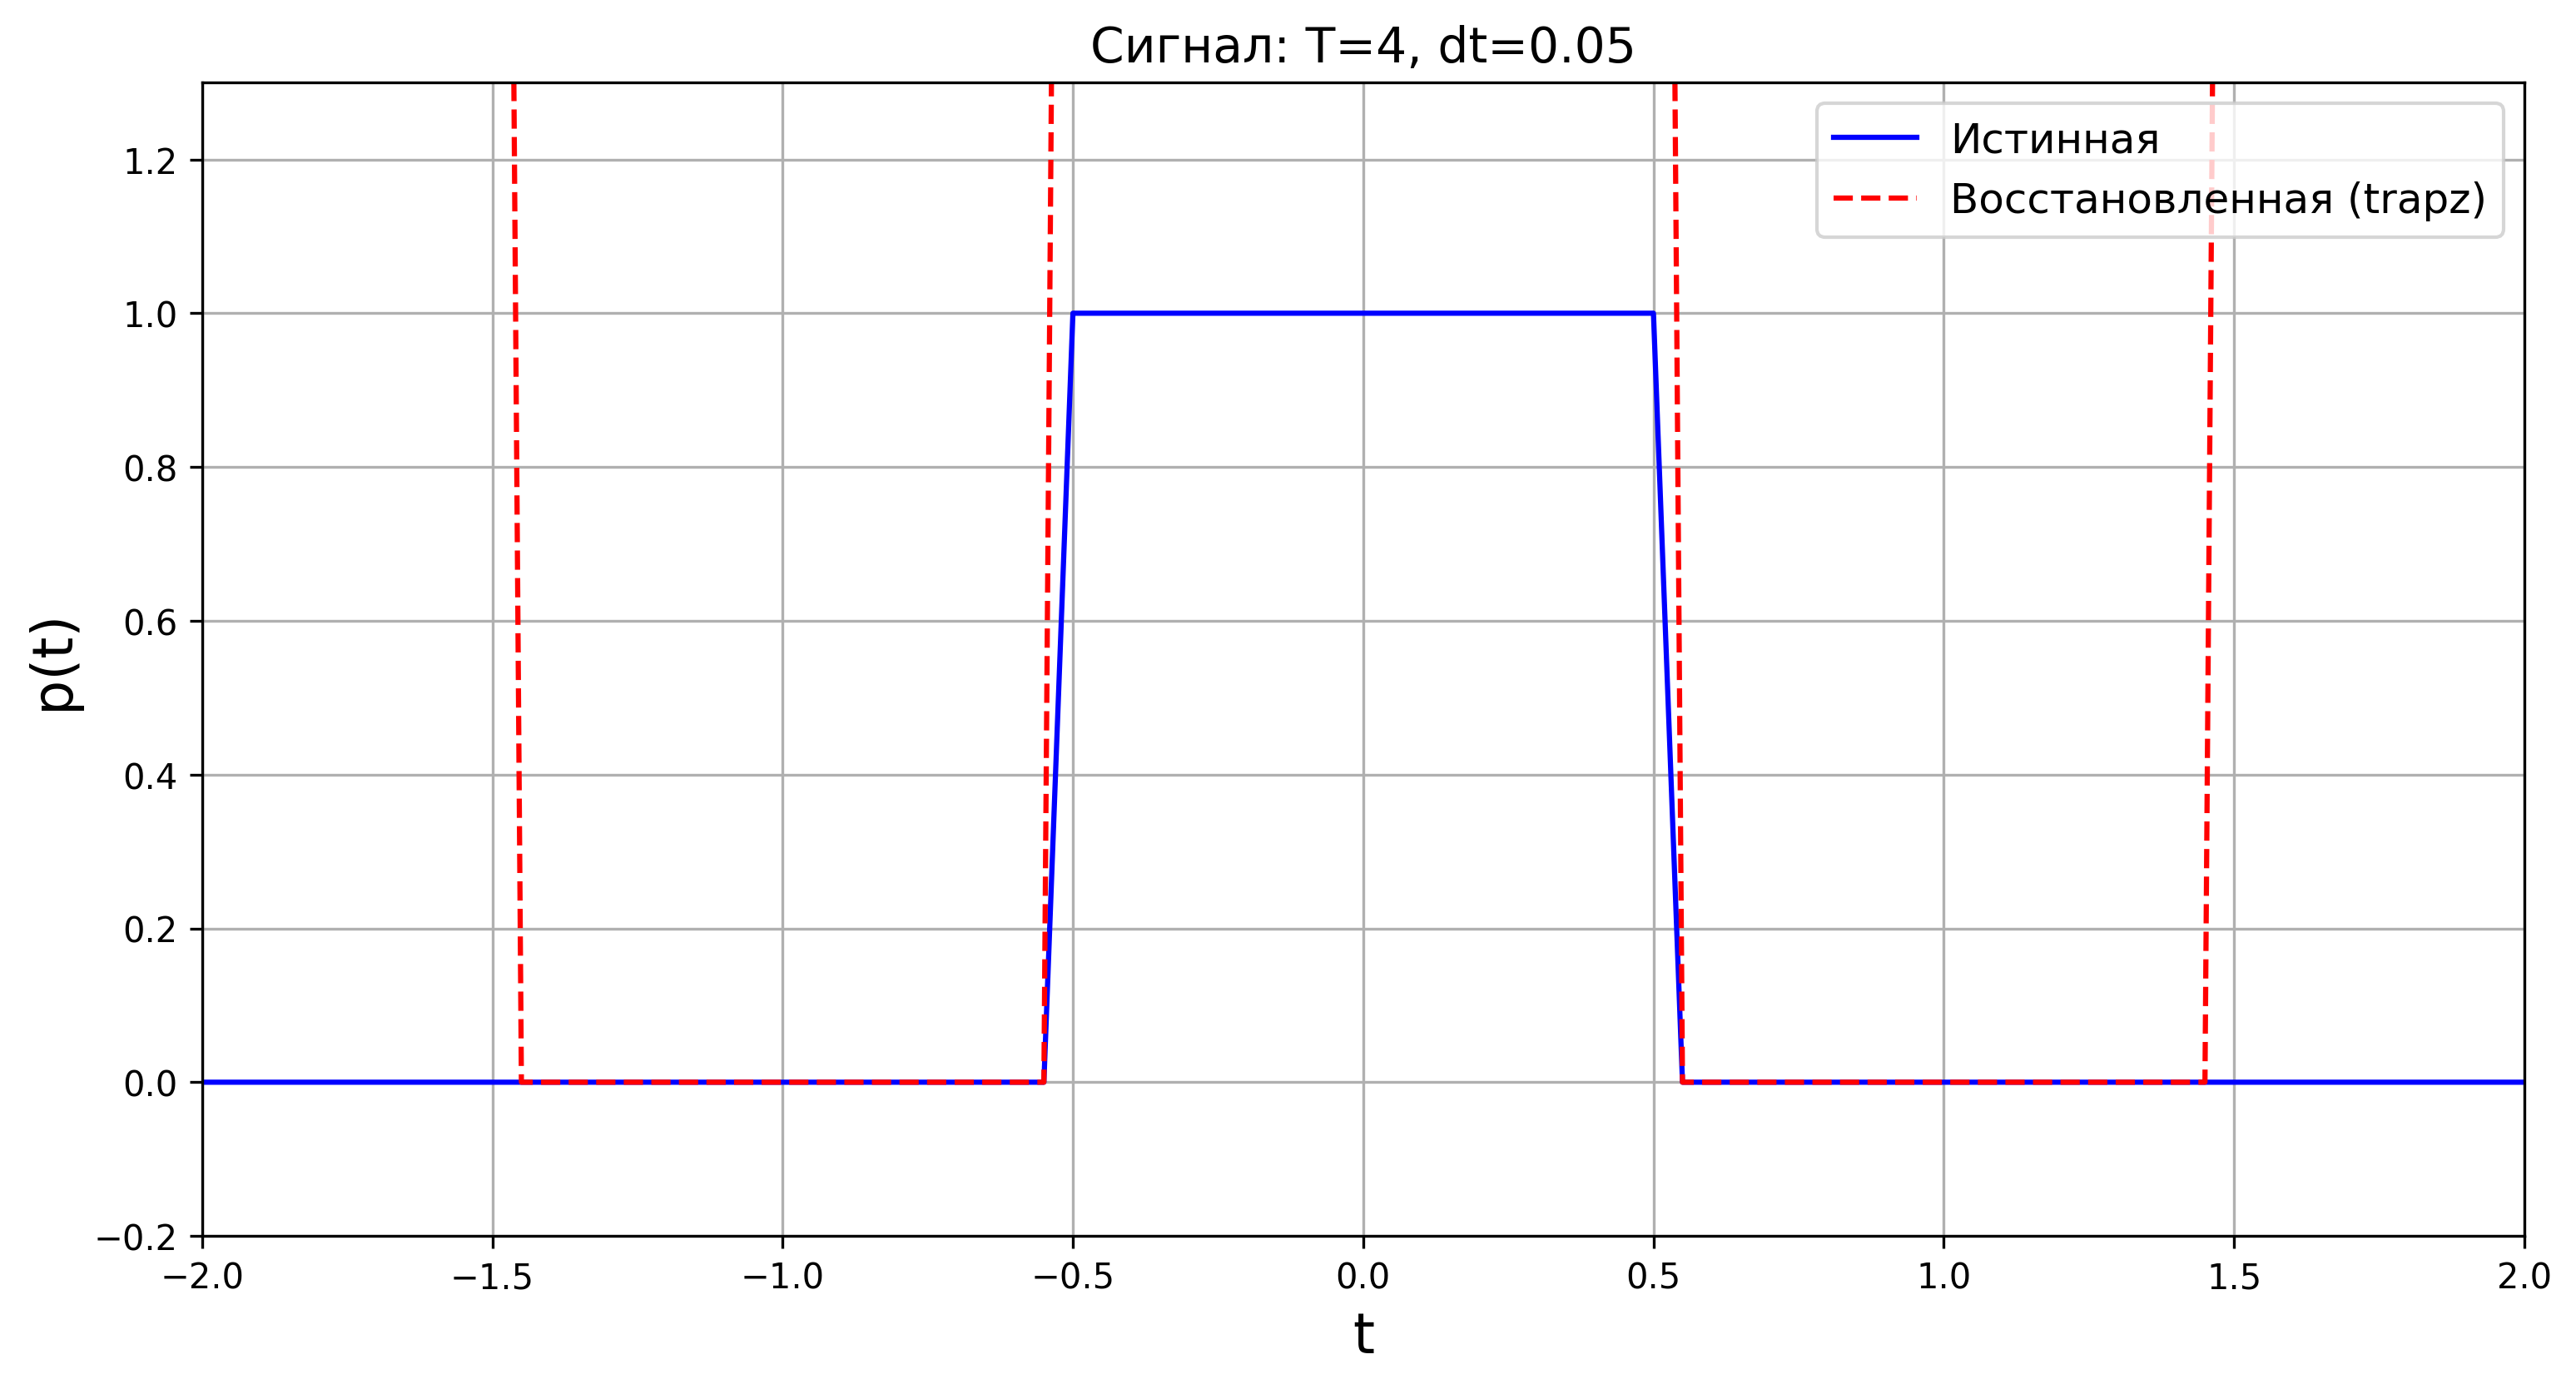
\includegraphics[width=0.95\textwidth]{Paper/images/T4_V100_dt0.050_dv0.500_signal.png}
    \caption{Сравнение исходной (синяя) и восстановленной (красная пунктир) функций.}
    \label{fig:signal_5}
\end{figure}

\begin{figure}[H]
    \centering
    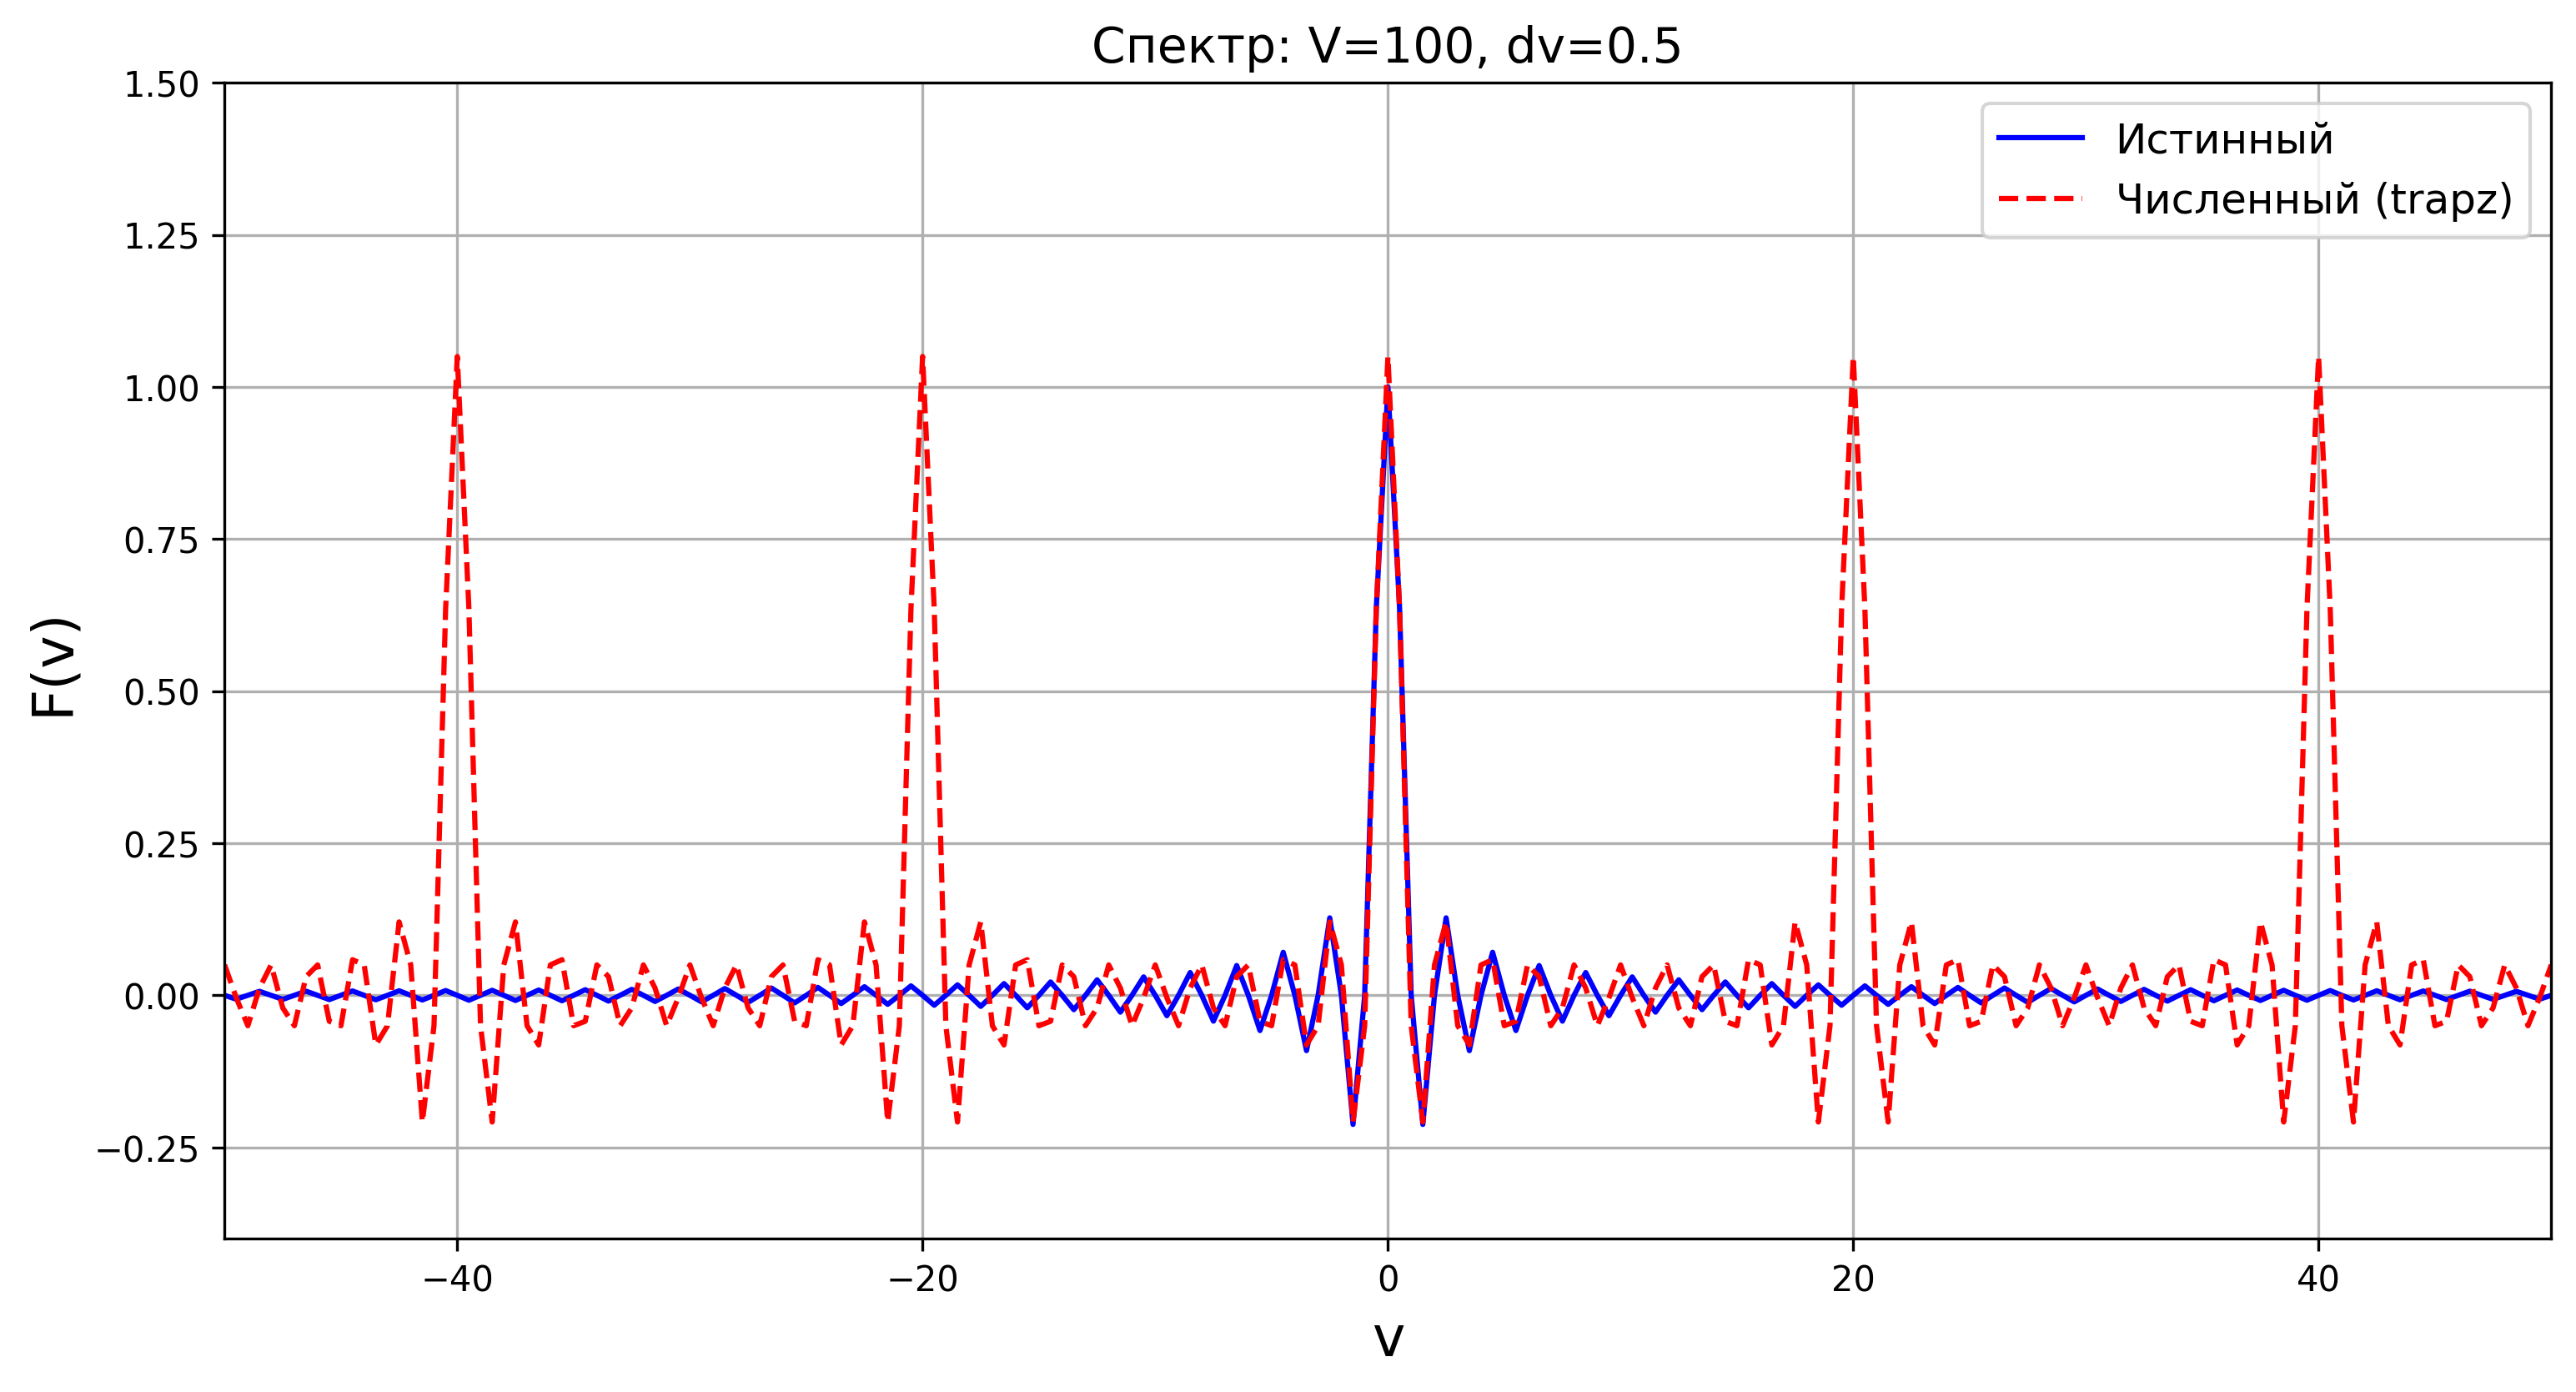
\includegraphics[width=0.95\textwidth]{Paper/images/T4_V100_dt0.050_dv0.500_spectrum.png}
    \caption{Сравнение истинного (синяя) и численного (красная пунктир) спектров.}
    \label{fig:spectrum_5}
\end{figure}


\newpage
\subsection{Комбинация 6: $T=8$, $V=200$, $dt=0.050$, $dv=0.500$}

\begin{figure}[H]
    \centering
    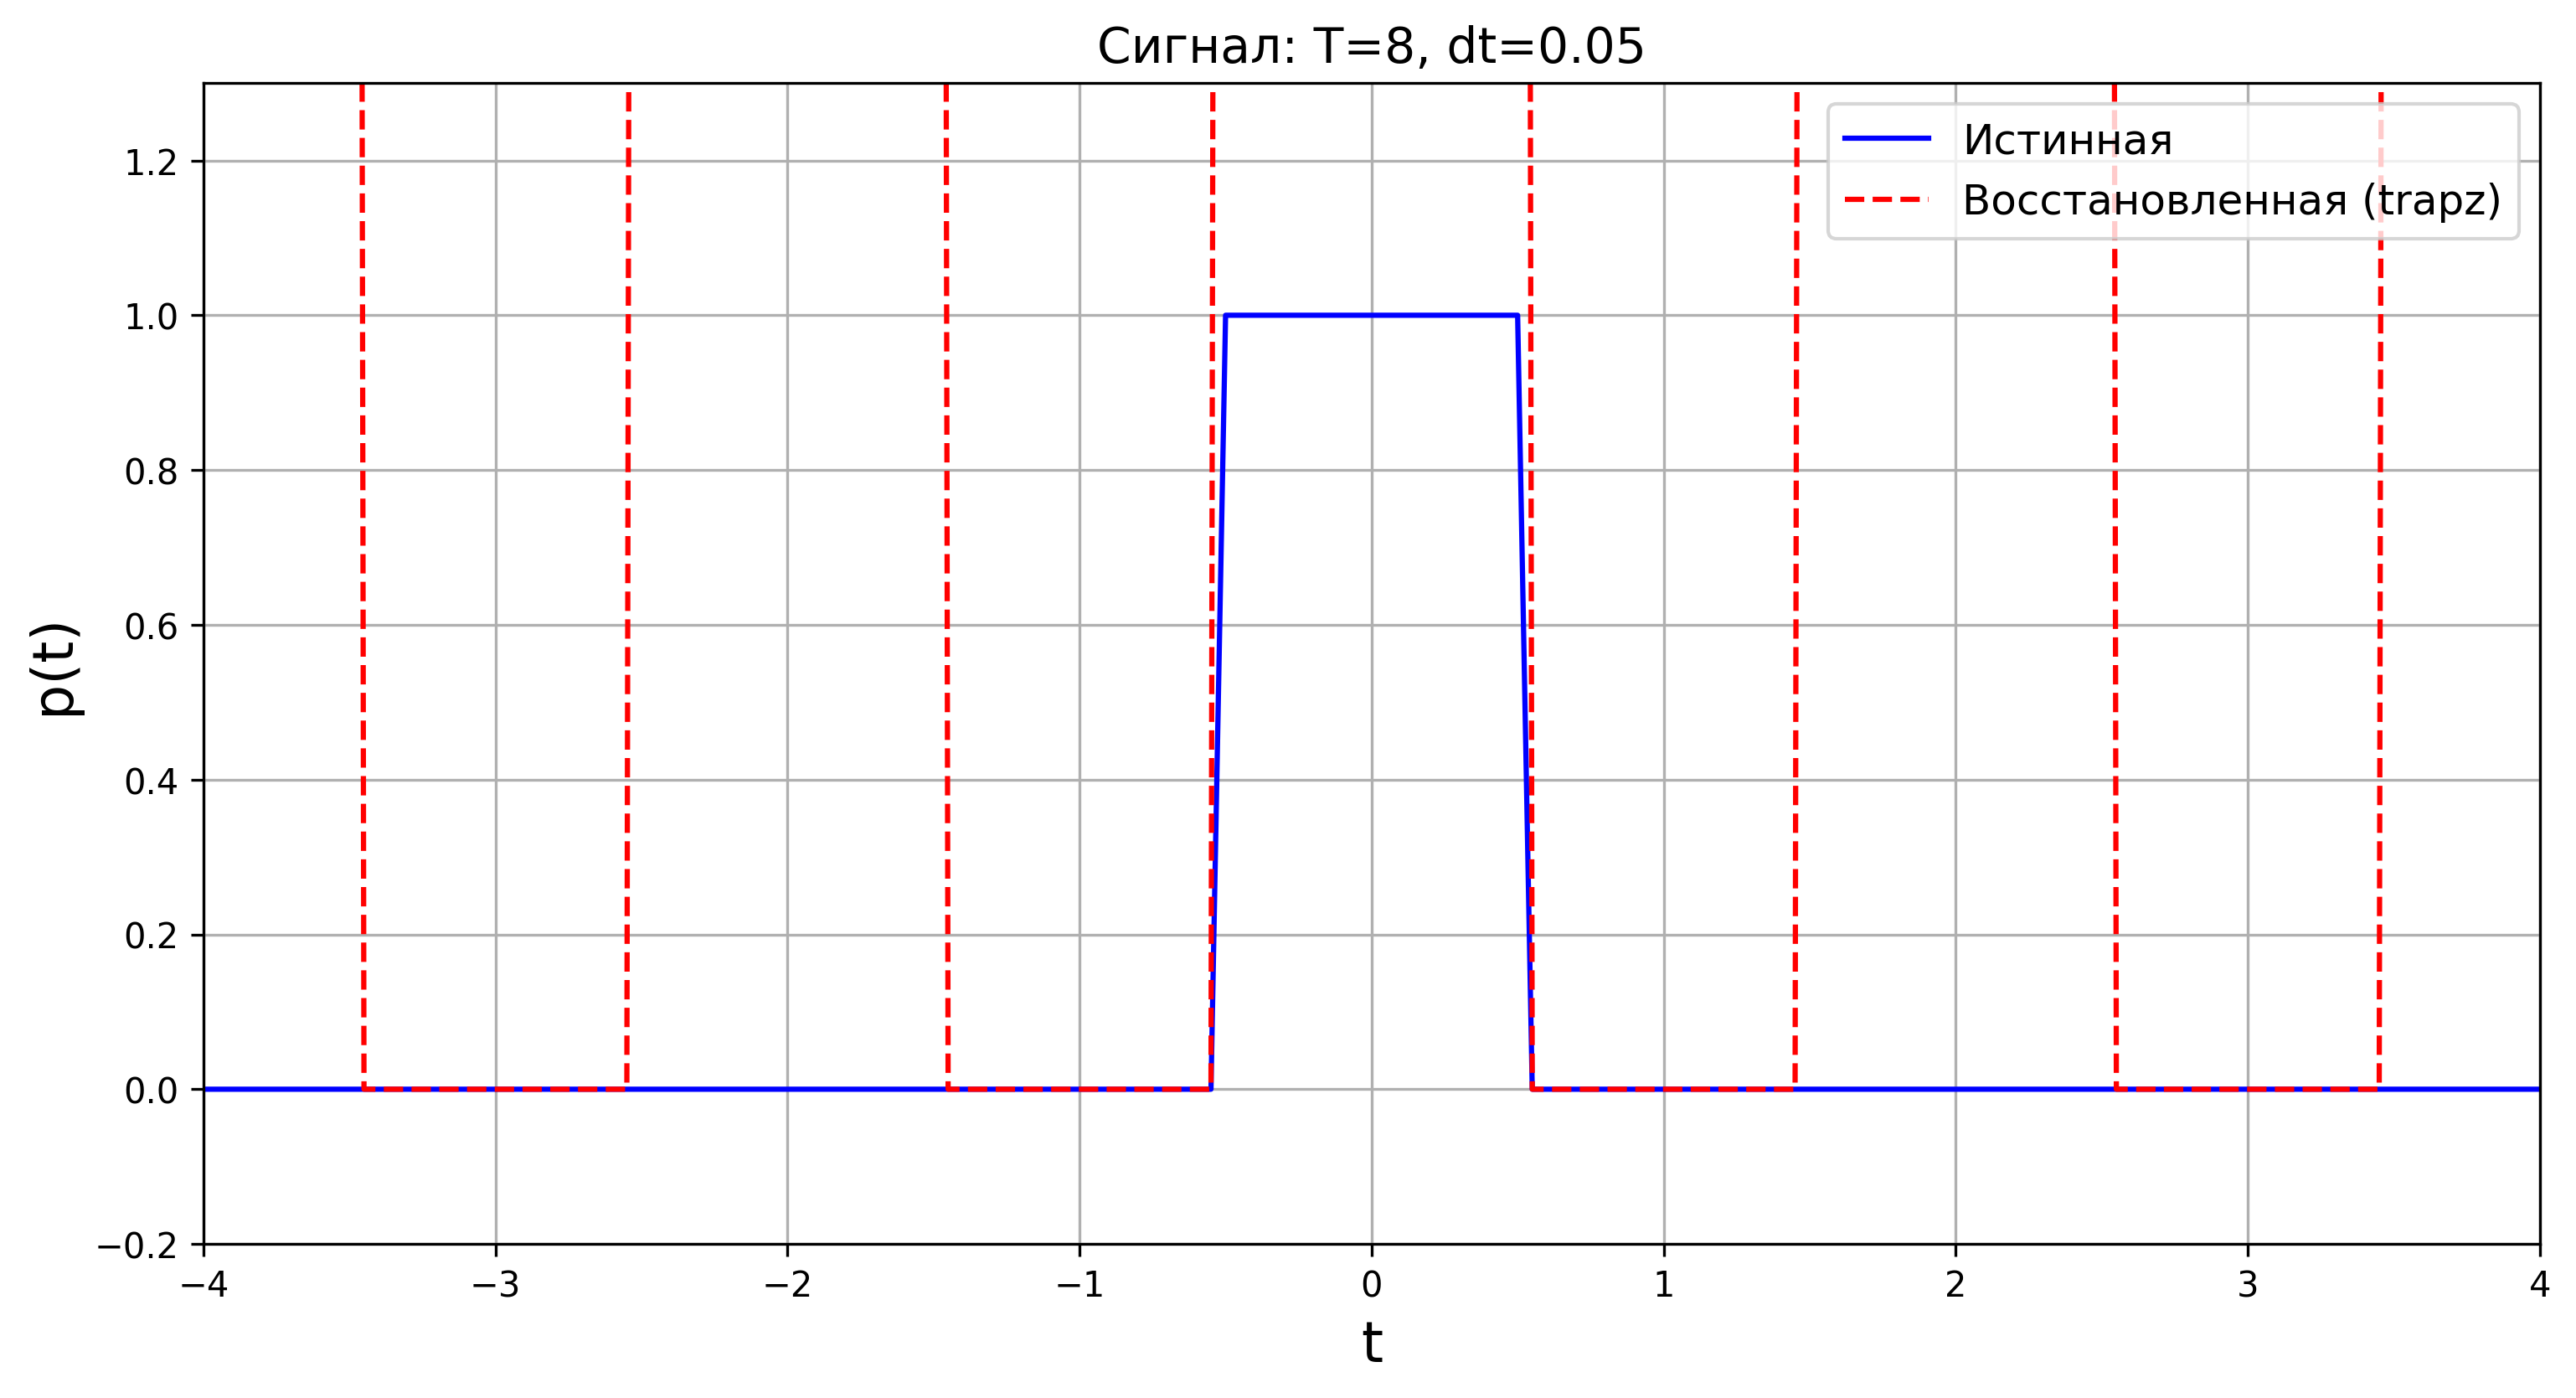
\includegraphics[width=0.95\textwidth]{Paper/images/T8_V200_dt0.050_dv0.500_signal.png}
    \caption{Сравнение исходной (синяя) и восстановленной (красная пунктир) функций.}
    \label{fig:signal_6}
\end{figure}

\begin{figure}[H]
    \centering
    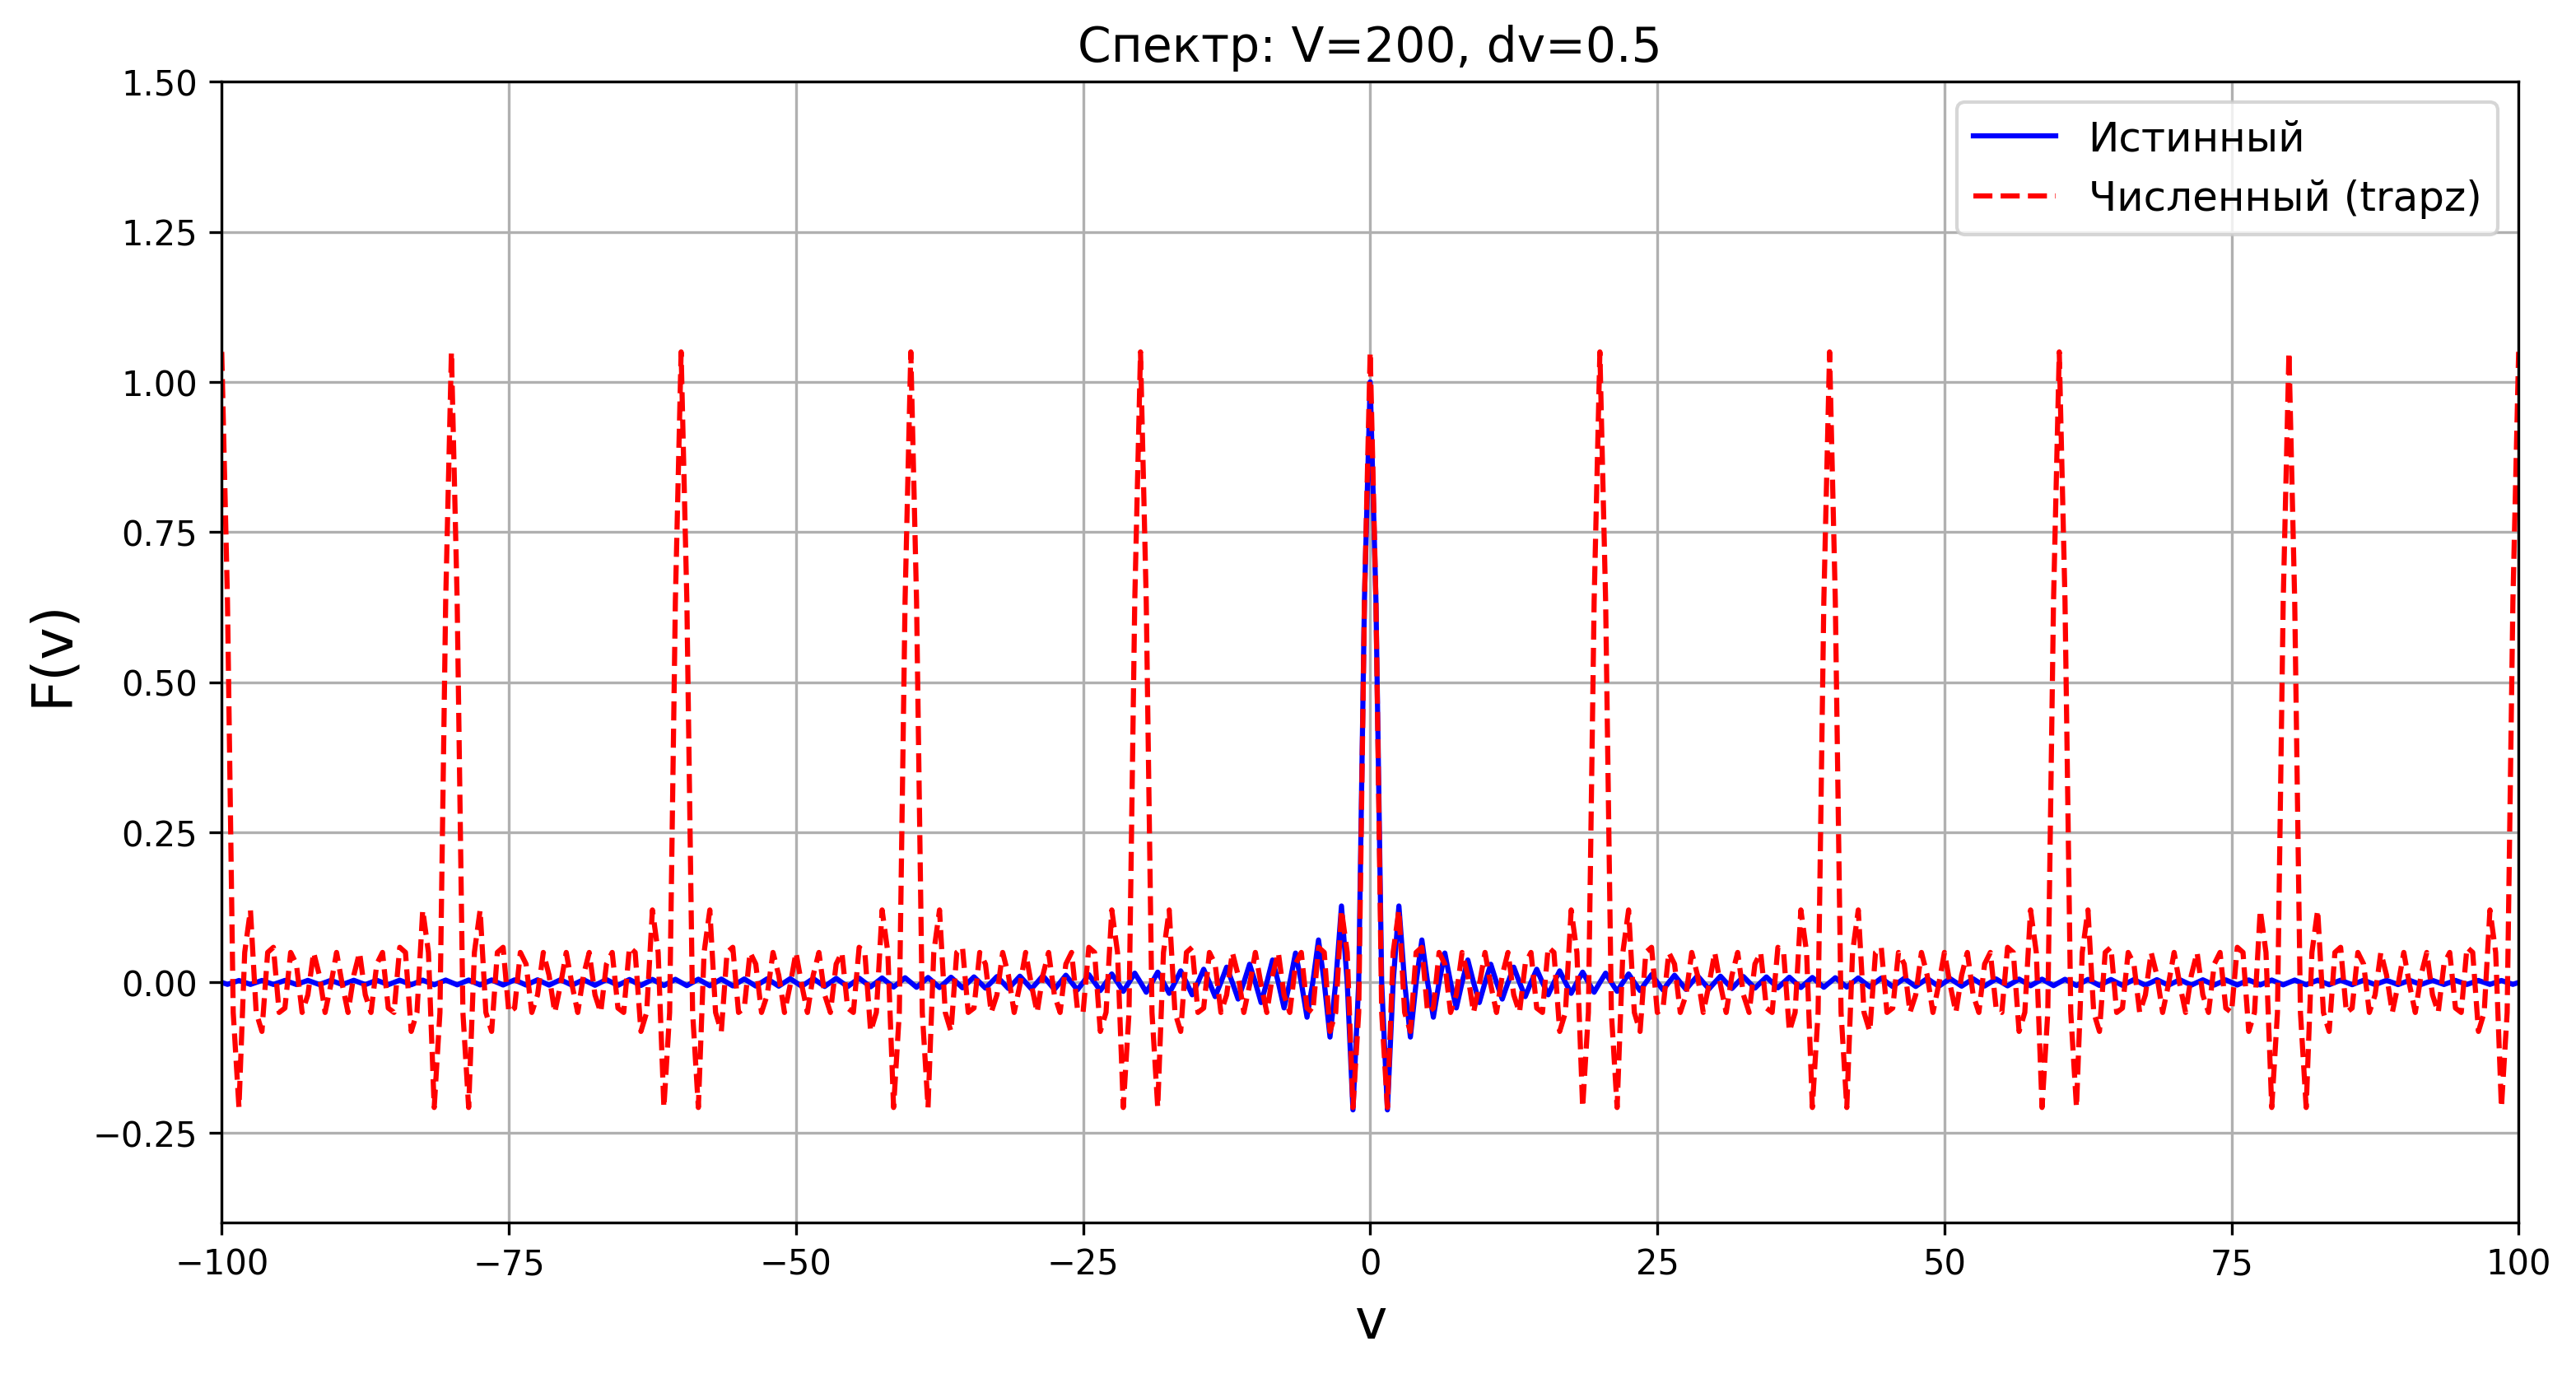
\includegraphics[width=0.95\textwidth]{Paper/images/T8_V200_dt0.050_dv0.500_spectrum.png}
    \caption{Сравнение истинного (синяя) и численного (красная пунктир) спектров.}
    \label{fig:spectrum_6}
\end{figure}


\newpage
\subsection{Комбинация 7: $T=4$, $V=100$, $dt=0.030$, $dv=0.250$}

\begin{figure}[H]
    \centering
    \includegraphics[width=0.95\textwidth]{Paper/images/T4_V100_dt0.030_dv0.250_signal.png}
    \caption{Сравнение исходной (синяя) и восстановленной (красная пунктир) функций.}
    \label{fig:signal_7}
\end{figure}

\begin{figure}[H]
    \centering
    \includegraphics[width=0.95\textwidth]{Paper/images/T4_V100_dt0.030_dv0.250_spectrum.png}
    \caption{Сравнение истинного (синяя) и численного (красная пунктир) спектров.}
    \label{fig:spectrum_7}
\end{figure}

